% !Mode::"TeX:UTF-8"
% !Mode:: "TeX:UTF-8"
\documentclass[xcolor=svgnames,serif,table,10pt]{beamer}
\mode<presentation>{
% Setup appearance:
\usecolortheme[named=FireBrick]{structure}
\useoutertheme{infolines}
\usetheme{Darmstadt}
\setbeamercovered{transparent}
\setbeamertemplate{caption}[numbered]
\setbeamertemplate{navigation symbols}{}
\setbeamertemplate{blocks}[rounded][shadow=true]
\setbeamertemplate{enumerate items}[circle]

% 修改样式
\setbeamercolor{box}{bg=black!20!orange,fg=white}
\setbeamercolor{block title}{use=sidebar,fg=sidebar.fg!10!white,bg=orange!70!black}
\setbeamercolor{block title example}{use=sidebar,fg=sidebar.fg!10!white,bg=black!60!green}
\setbeamercolor{block title alerted}{use=sidebar,fg=sidebar.fg!10!white,bg=black!50!red}

\setbeamertemplate{headline}
{%
  \begin{beamercolorbox}[shadow=true]{section in head/foot}
  \vskip2pt\insertnavigation{\paperwidth}\vskip2pt
  \end{beamercolorbox}%
}
}
\usepackage[english]{babel}
\usepackage{times}
\usepackage[T1]{fontenc}
\usepackage{multirow,multicol,longtable}
\usepackage{graphics}
\usepackage{xcolor}
\usepackage[no-math]{fontspec}%--------------------------------------------------提供字体选择命令
\usepackage{xunicode}%-----------------------------------------------------------提供Unicode字符宏
\usepackage{xltxtra}%------------------------------------------------------------提供了针对XeTeX的改进并且加入了XeTeX的LOGO
\usepackage[BoldFont,SlantFont,CJKchecksingle]{xeCJK}%---------------------------使用xeCJK宏包
%================================== 设置中文字体 ================================%
\setCJKmainfont{Adobe Heiti Std}%------------------------------------------------设置正文为黑体
\setCJKmonofont{Adobe Song Std}%-------------------------------------------------设置等距字体
\setCJKsansfont{Adobe Kaiti Std}%------------------------------------------------设置无衬线字体
% \setCJKfamilyfont{zxzt}{FZShouJinShu-S10S}
% \setCJKfamilyfont{FZDH}{FZDaHei-B02S}
%================================== 设置中文字体 ================================%

%================================== 设置英文字体 ================================%
\setmainfont[Mapping=tex-text]{Times New Roman}%--------------------------------英文衬线字体
\setsansfont[Mapping=tex-text]{Arial}%------------------------------------英文无衬线字体
\setmonofont[Mapping=tex-text]{Courier New}%-------------------------------------英文等宽字体
\newfontfamily\Arial{Arial}
%================================== 设置英文字体 ================================%

%================================== 设置数学字体 ================================%
%\setmathsfont(Digits,Latin,Greek)[Numbers={Lining,Proportional}]{Minion Pro}
%================================== 设置数学字体 ================================%
\punctstyle{kaiming}%------------------------------------------------------------开明式标点格式
\usepackage{graphicx}
\usepackage{tikz}
\usetikzlibrary{positioning,backgrounds}
\usetikzlibrary{fadings}
\usetikzlibrary{patterns}
\usetikzlibrary{calc}
\usetikzlibrary{shadings}
\pgfdeclarelayer{background}
\pgfdeclarelayer{foreground}
\pgfsetlayers{background,main,foreground}
\usepackage{xifthen}
\usepackage{colortbl,dcolumn}
\usepackage{enumerate}
\usepackage{pifont}
\usepackage{tabularx}
\usepackage{booktabs}

%=================================== 数学符号 =================================%
\newcommand{\rtn}{\mathrm{\mathbf{R}}}
\newcommand{\N}{\mathrm{\mathbf{N}}}
\newcommand{\As}{\mathrm{a.s.}}
\newcommand{\Ae}{\mathrm{a.e.}}
\newcommand*{\PR}{\mathrm{\mathbf{P}}}
\newcommand*{\EX}{\mathrm{\mathbf{E}}}
\newcommand{\EXlr}[1]{\mathrm{\mathbf{E}}\left[#1\right]}
\newcommand*{\dif}{\,\mathrm{d}}
\newcommand*{\F}{\mathcal{F}}
\newcommand*{\h}{\mathcal{H}}
\newcommand*{\vp}{\varepsilon}
\newcommand*{\prs}{\dif\PR-\As}
\newcommand*{\dte}{\dif t-\Ae}
\newcommand*{\pts}{\dif\PR\times\dif t-\Ae}
\newcommand{\Ito}{It\^{o}}
\newcommand{\tT}[1][0]{[#1,T]}
\newcommand{\intT}[2][T]{\int^{#1}_{#2}}
\newcommand{\intTe}[1][t]{\intT[t+\varepsilon]{#1}}
\newcommand{\s}{\mathcal{S}}
\newcommand{\me}{\mathrm{e}}
\newcommand{\one}[1]{{\bf 1}_{#1}}
\renewcommand{\M}{{\rm M}}
\newcommand{\Me}[1][t]{M^{\varepsilon}_{#1}}
\newcommand{\Ne}[1][t]{N^{\varepsilon}_{#1}}
\newcommand{\Pe}[1][t]{P^{\varepsilon}_{#1}}
\DeclareMathOperator*{\sgn}{sgn}
% =================================== 数学符号 =================================%

% 定义罗马数字
\makeatletter
\newcommand{\rmnum}[1]{\romannumeral #1}
\newcommand{\Rmnum}[1]{\expandafter\@slowromancap\romannumeral #1@}
\makeatother

% 定义破折号
\newcommand{\pozhehao}{\kern0.3ex\rule[0.8ex]{2em}{0.1ex}\kern0.3ex}
% 中文日期
\def\CJK@today{\the\year 年 \the\month 月}
\newcommand\zhtoday{\CJK@today}

% 中文图表
\renewcommand\figurename{图}
\renewcommand\tablename{表}

\graphicspath{{figures/}}

% Author, Title, etc.

\title{前景约束的欧拉影像动作放大技术}

\subtitle{Foreground-constrained Eulerian Video Motion Magnification}

\author[潘伟洲]{姓名:\makebox[4em][s]{潘伟洲~\hspace{2em}}\\
  导师:\makebox[4em][s]{李兴民~教授}\\
  专业:\makebox[4em][s]{计算应用技术}\\
  方向:\makebox[4em][s]{数字图像处理}}

\institute[SCNU]{
\includegraphics[height=1cm]{scnu.jpg}\\ 2014届硕士学位论文答辩}

\date{\tiny 2013-05-25}

\setlength{\baselineskip}{22pt}
\renewcommand{\baselinestretch}{1.4}

% The main document

\begin{document}

\setlength{\abovedisplayskip}{1ex}%------------------------------------------ 公式前的距离
\setlength{\belowdisplayskip}{1ex}%------------------------------------------ 公式后的距离

\begin{frame}
  \titlepage
\end{frame}

\begin{frame}
  \frametitle{内容提纲}
  \vspace{-2.5em}
  \begin{figure}
    \centering
    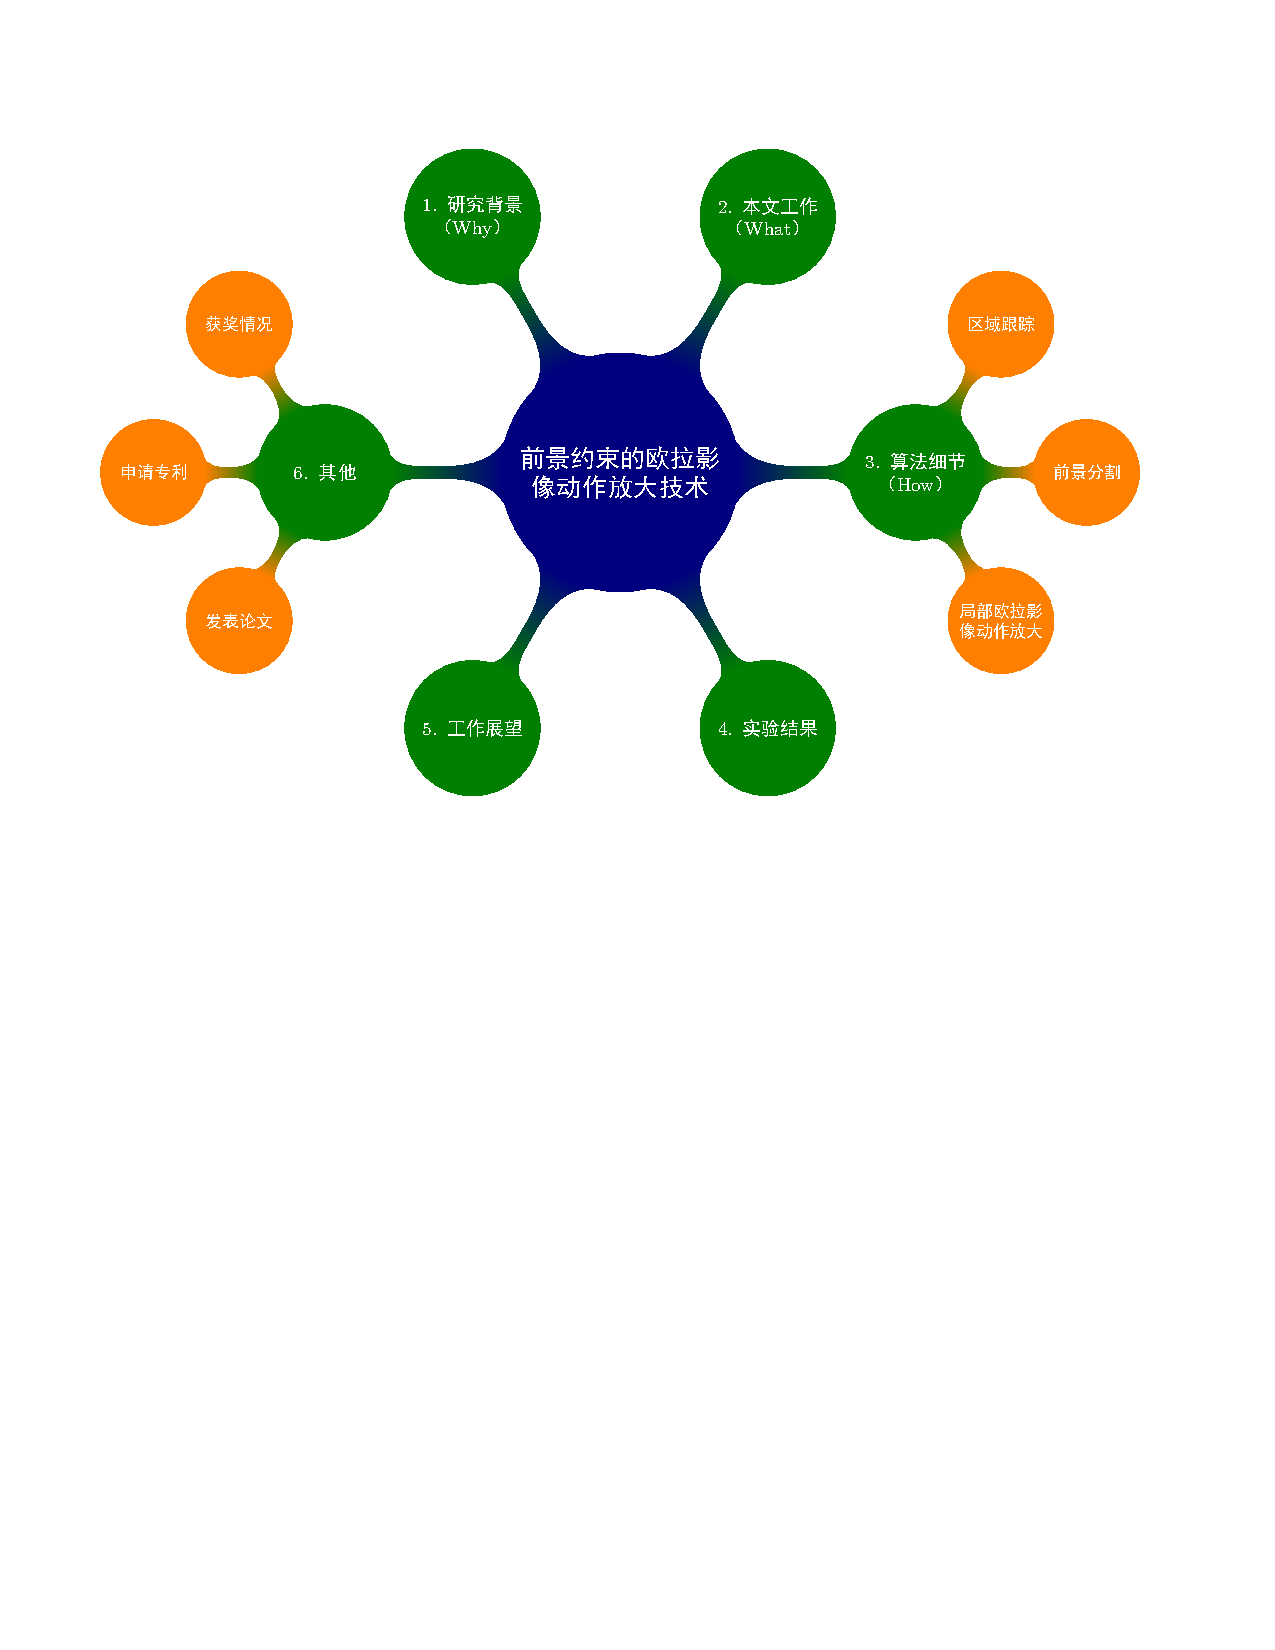
\includegraphics[width=\textwidth, page=1]{mindmap.pdf}
  \end{figure}
\end{frame}

\section{研究背景}
\label{sec:Why}

\begin{frame}{研究背景(Why)}
  \vspace{-2.5em}
  \begin{figure}
    \centering
    \includegraphics[width=\textwidth, page=2]{mindmap.pdf}
  \end{figure}
\end{frame}

\begin{frame}
  \frametitle{研究背景(Why)}
  人类的视觉感知系统存在有限的感知域。对于超出感知域的微弱变化,裸眼无法感知。然
  而,这类信号却可能带有重要的信息。

  \medskip
  \begin{center}
    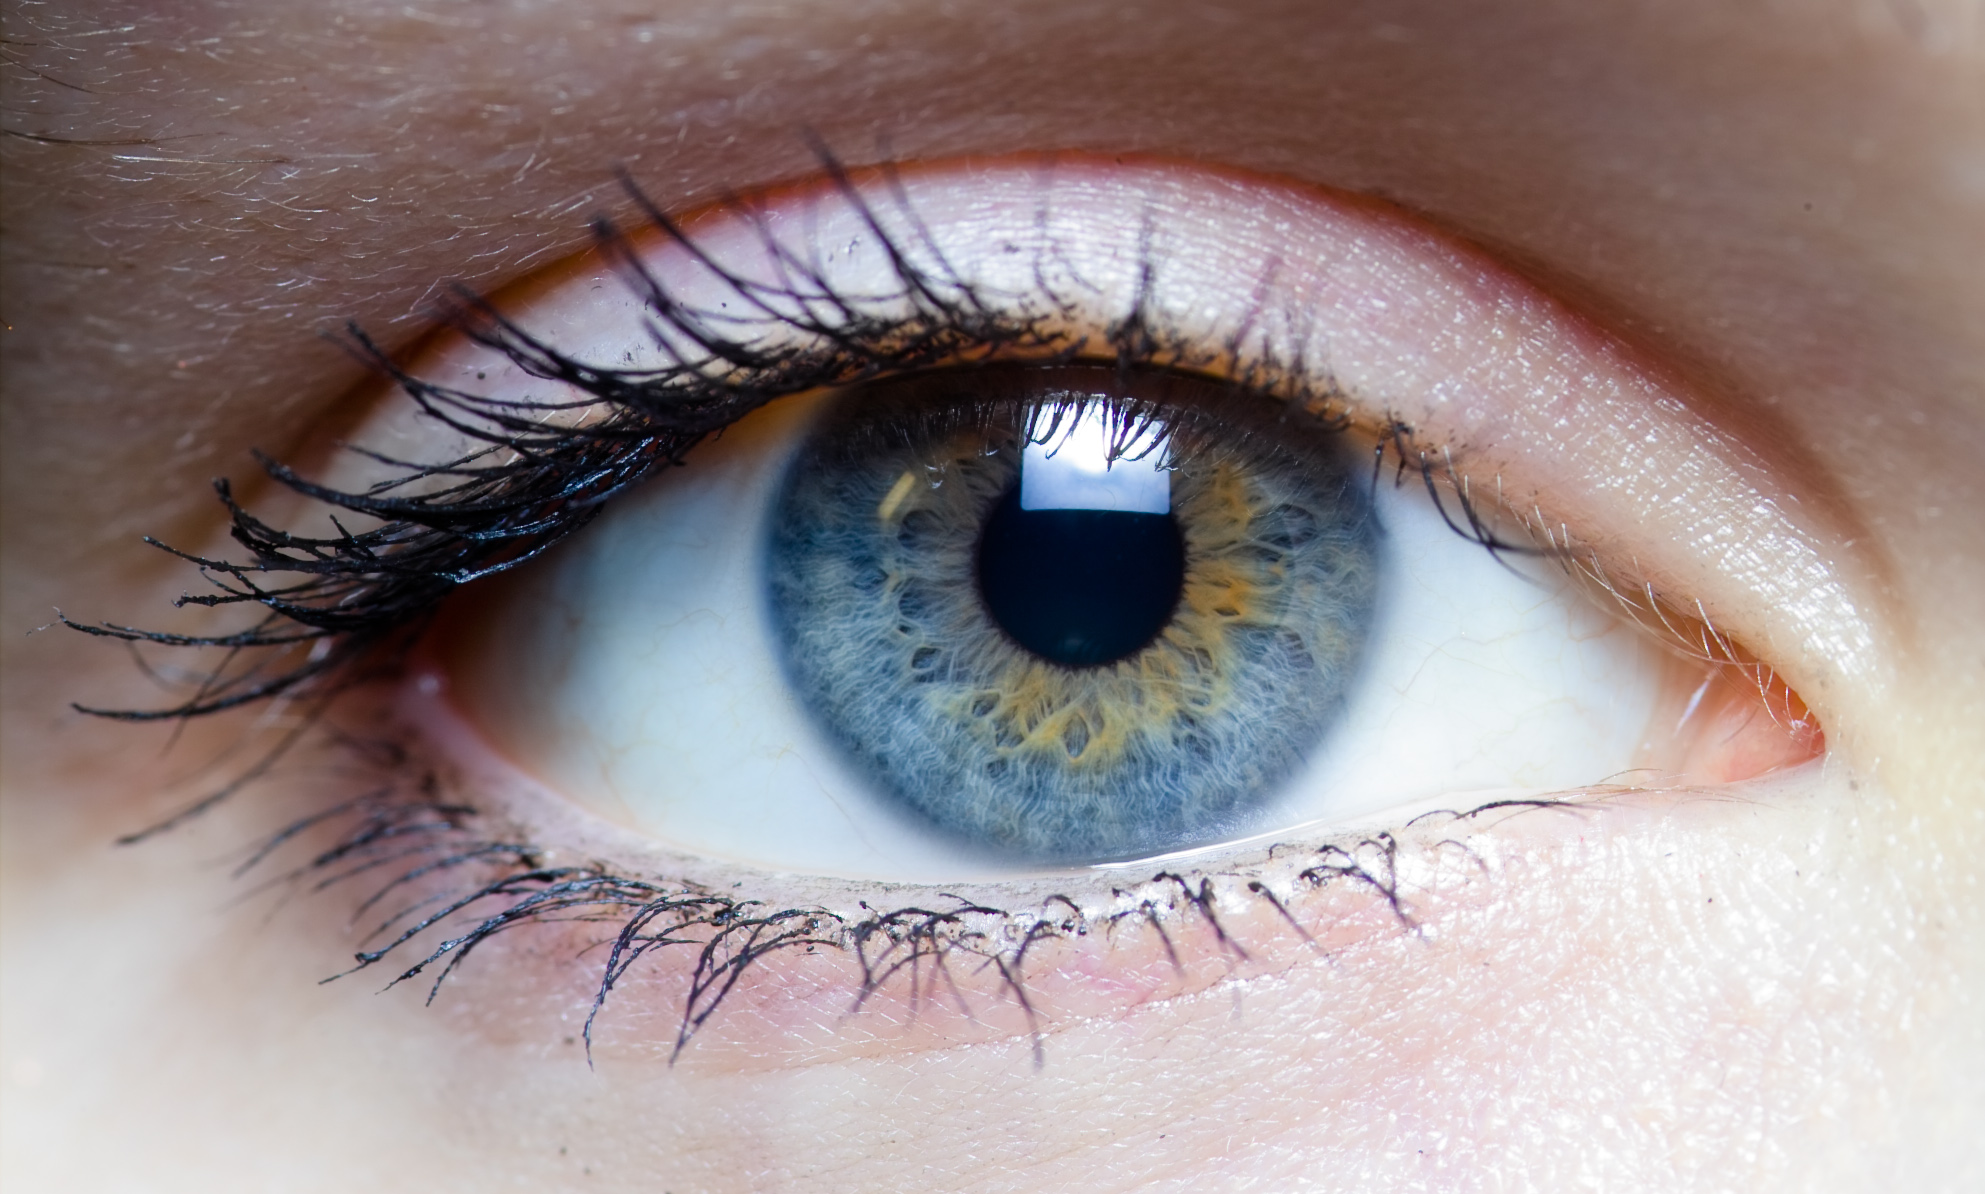
\includegraphics[width=.5\textwidth]{eye.jpg}
  \end{center}
\end{frame}

\begin{frame}
  \frametitle{Mingzhe Poh的“魔镜”}
  \small
  2011 年,MIT 的一个亚裔学生 Mingzhe Poh 利用了血液在人体内流动导致皮肤表面反射
  光线的微弱变化设计了一面可以测量心率的“镜子”\cite{poh2011medical}。

  \medskip
\begin{center}
    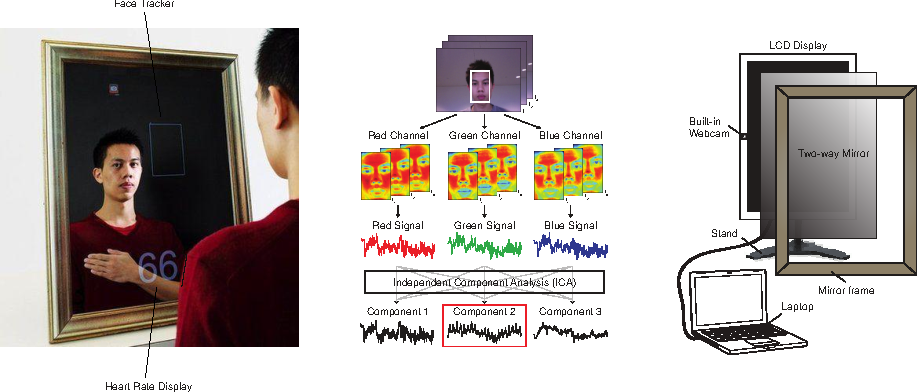
\includegraphics[width=\textwidth]{mirror.pdf}
  \end{center}
\end{frame}

\begin{frame}[t]
  \frametitle{细微变化的价值}
  \begin{center}
  \only<1>{
  \begin{tikzpicture}
    \draw[draw=white] (0,0) .. controls (3,1.3) and (6,1.3) .. (9,0)
    node[pos=0,sloped,draw=orange,inner sep=.1mm]
      {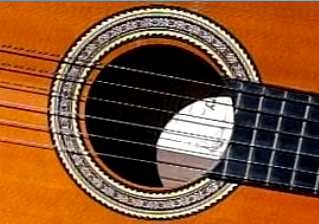
\includegraphics[height=2cm]{guitar.png}}
    node[pos=0.2,sloped,draw=orange,inner sep=.1mm,opacity=0]
      {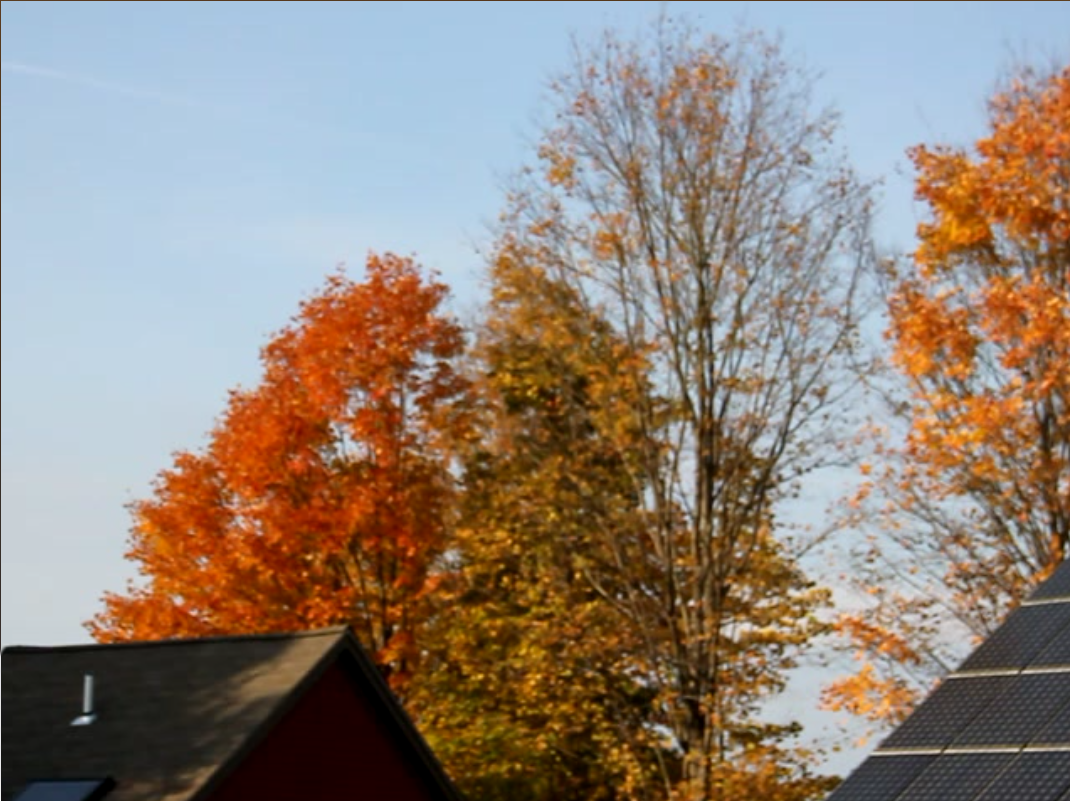
\includegraphics[height=2cm]{trees.png}}
    node[pos=0.4,sloped,draw=orange,inner sep=.1mm,opacity=0]
      {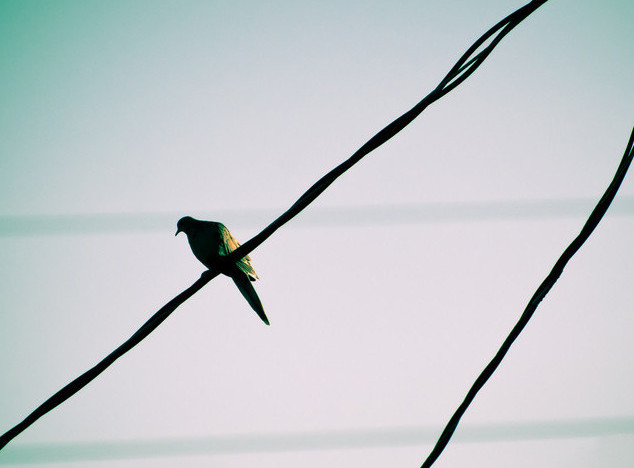
\includegraphics[height=2cm]{birds.jpg}}
    node[pos=0.6,sloped,draw=orange,inner sep=.1mm,opacity=0]
      {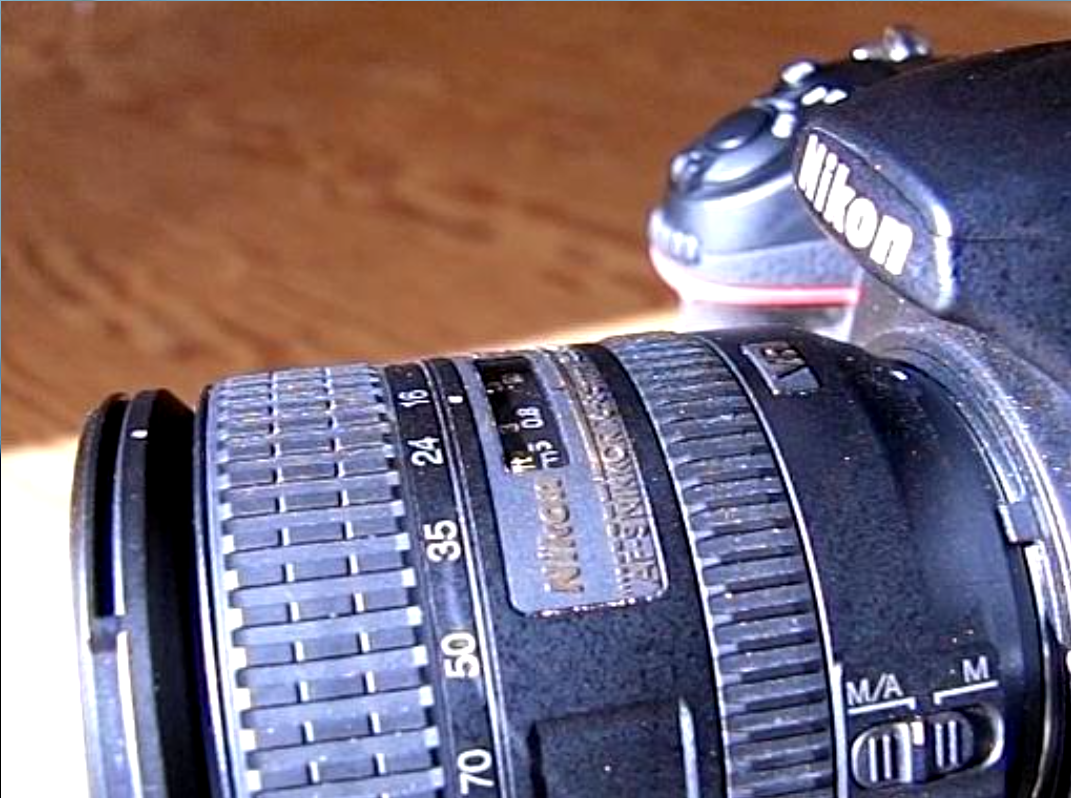
\includegraphics[height=2cm]{camera.png}}
    node[pos=0.8,sloped,draw=orange,inner sep=.1mm,opacity=0]
      {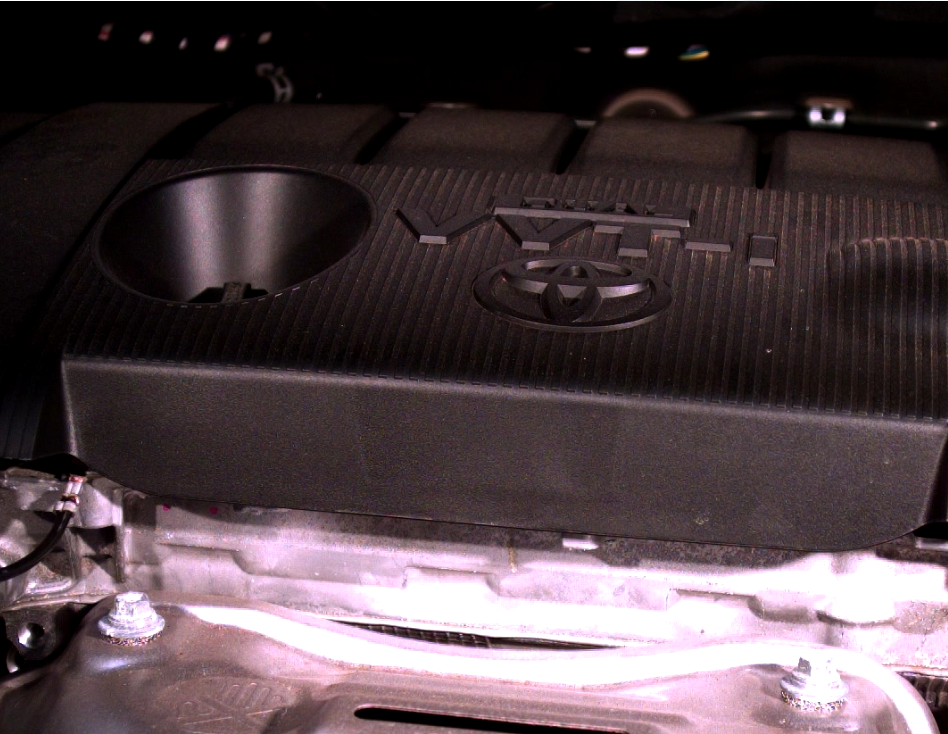
\includegraphics[height=2cm]{engine.png}}
    node[pos=1,sloped,draw=orange,inner sep=.1mm,opacity=0]
      {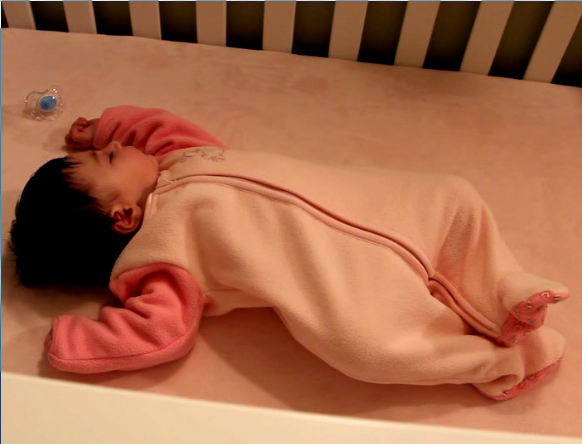
\includegraphics[height=2cm]{baby.png}};
    \end{tikzpicture}}
  \only<2>{
  \begin{tikzpicture}
    \draw[draw=white] (0,0) .. controls (3,1.3) and (6,1.3) .. (9,0)
    node[pos=0,sloped,draw=orange,inner sep=.1mm]
      {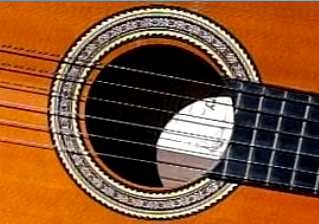
\includegraphics[height=2cm]{guitar.png}}
    node[pos=0.2,sloped,draw=orange,inner sep=.1mm]
      {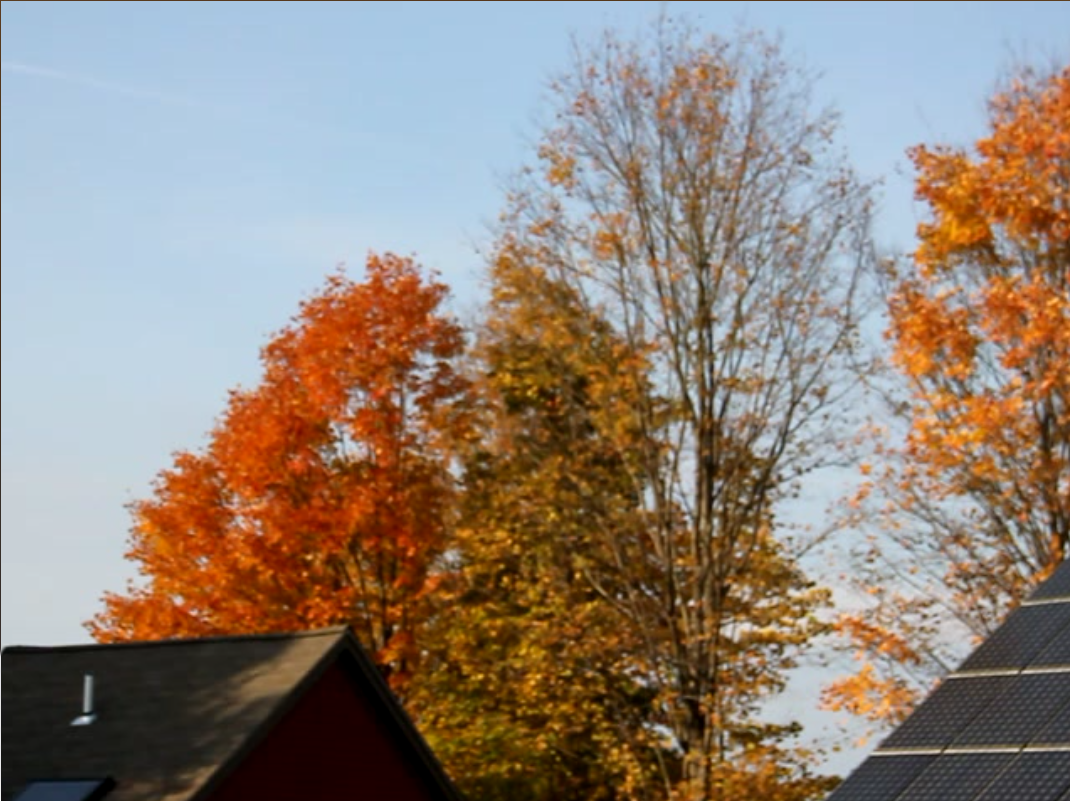
\includegraphics[height=2cm]{trees.png}}
    node[pos=0.4,sloped,draw=orange,inner sep=.1mm,opacity=0]
      {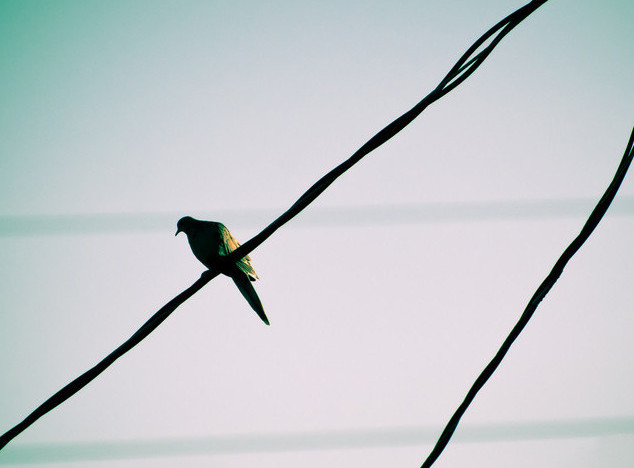
\includegraphics[height=2cm]{birds.jpg}}
    node[pos=0.6,sloped,draw=orange,inner sep=.1mm,opacity=0]
      {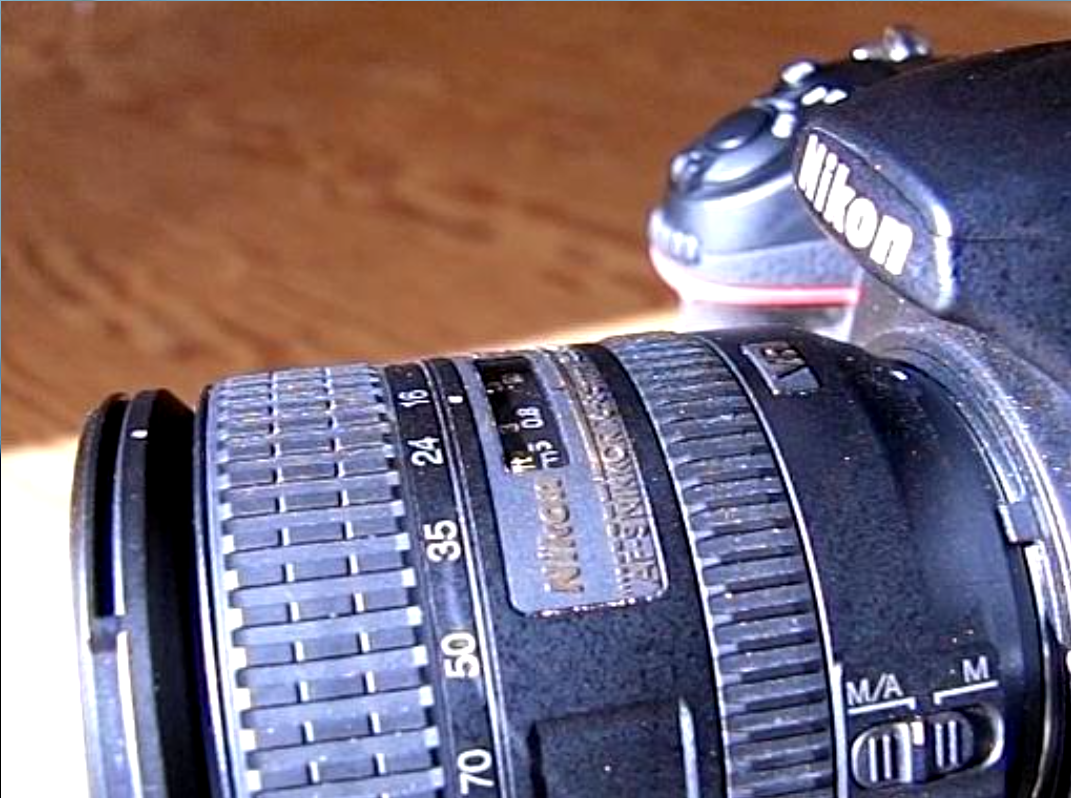
\includegraphics[height=2cm]{camera.png}}
    node[pos=0.8,sloped,draw=orange,inner sep=.1mm,opacity=0]
      {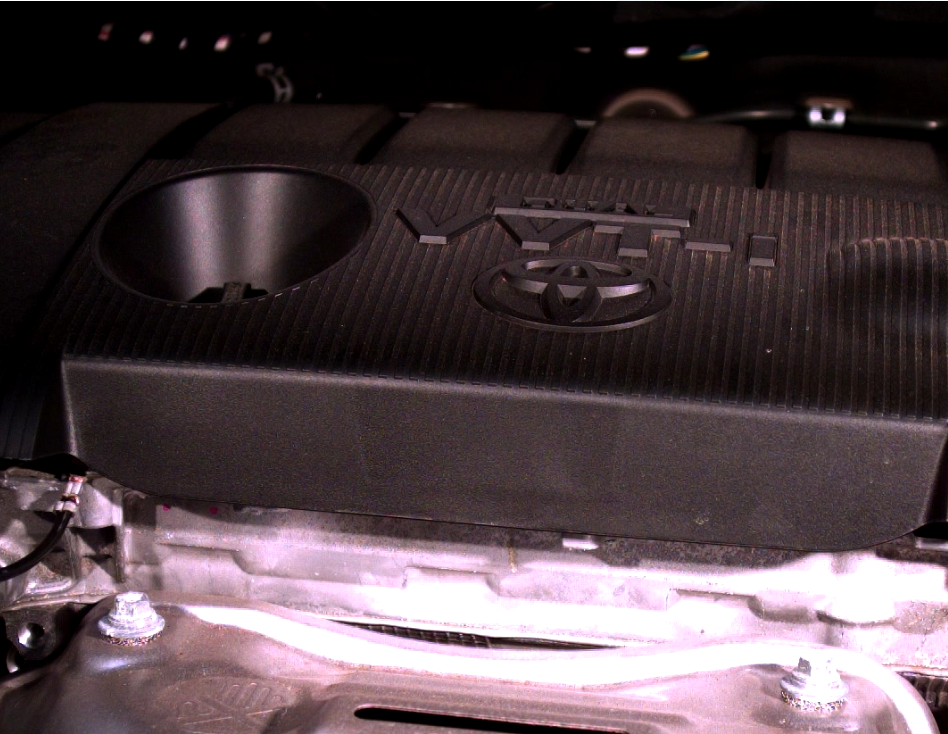
\includegraphics[height=2cm]{engine.png}}
    node[pos=1,sloped,draw=orange,inner sep=.1mm,opacity=0]
      {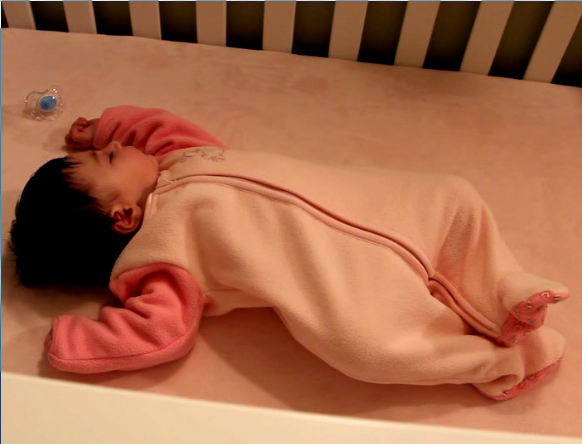
\includegraphics[height=2cm]{baby.png}};
    \end{tikzpicture}}
  \only<3>{
  \begin{tikzpicture}
    \draw[draw=white] (0,0) .. controls (3,1.3) and (6,1.3) .. (9,0)
    node[pos=0,sloped,draw=orange,inner sep=.1mm]
      {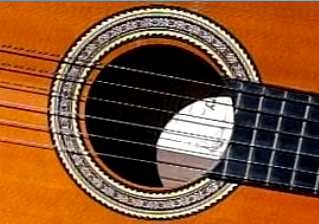
\includegraphics[height=2cm]{guitar.png}}
    node[pos=0.2,sloped,draw=orange,inner sep=.1mm]
      {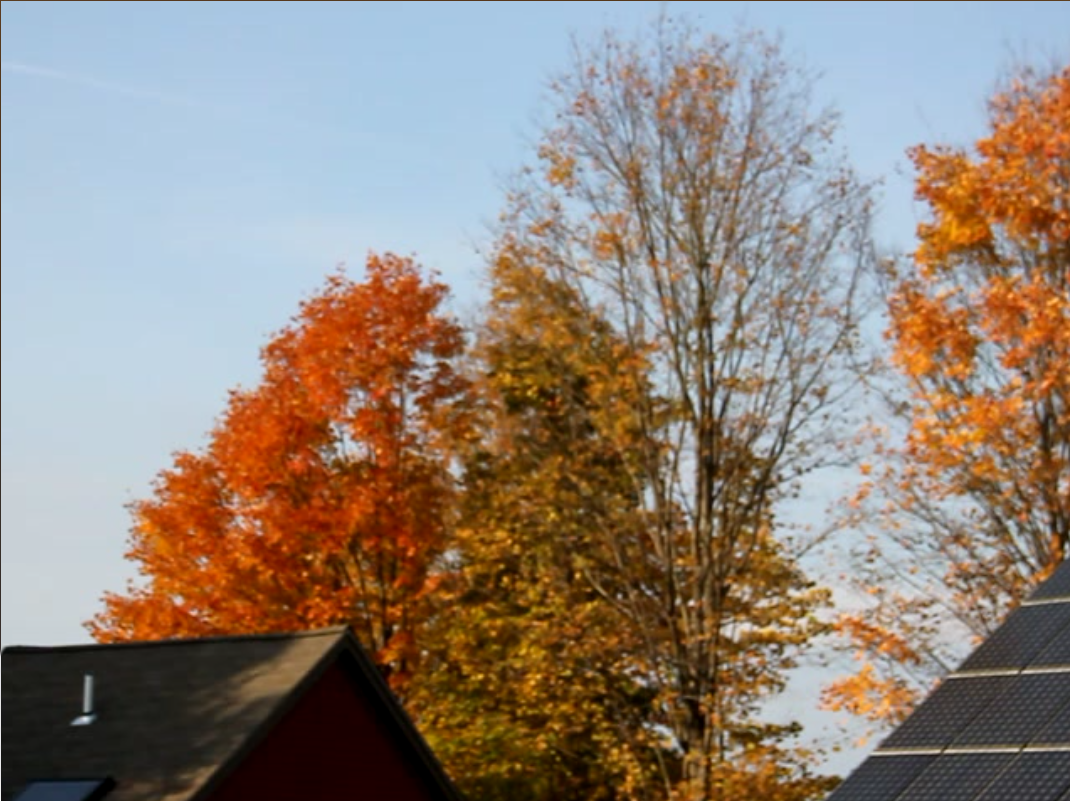
\includegraphics[height=2cm]{trees.png}}
    node[pos=0.4,sloped,draw=orange,inner sep=.1mm]
      {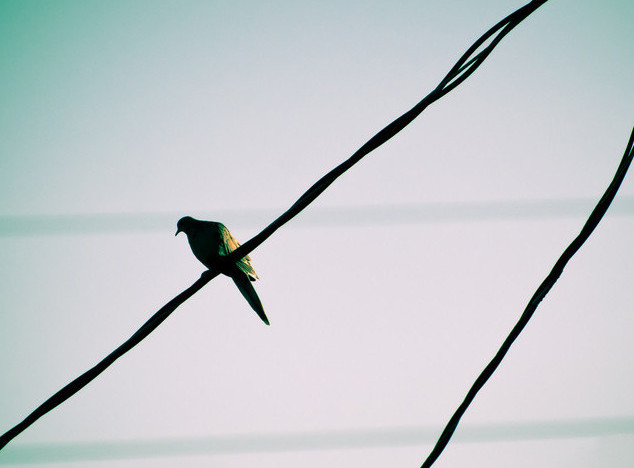
\includegraphics[height=2cm]{birds.jpg}}
    node[pos=0.6,sloped,draw=orange,inner sep=.1mm,opacity=0]
      {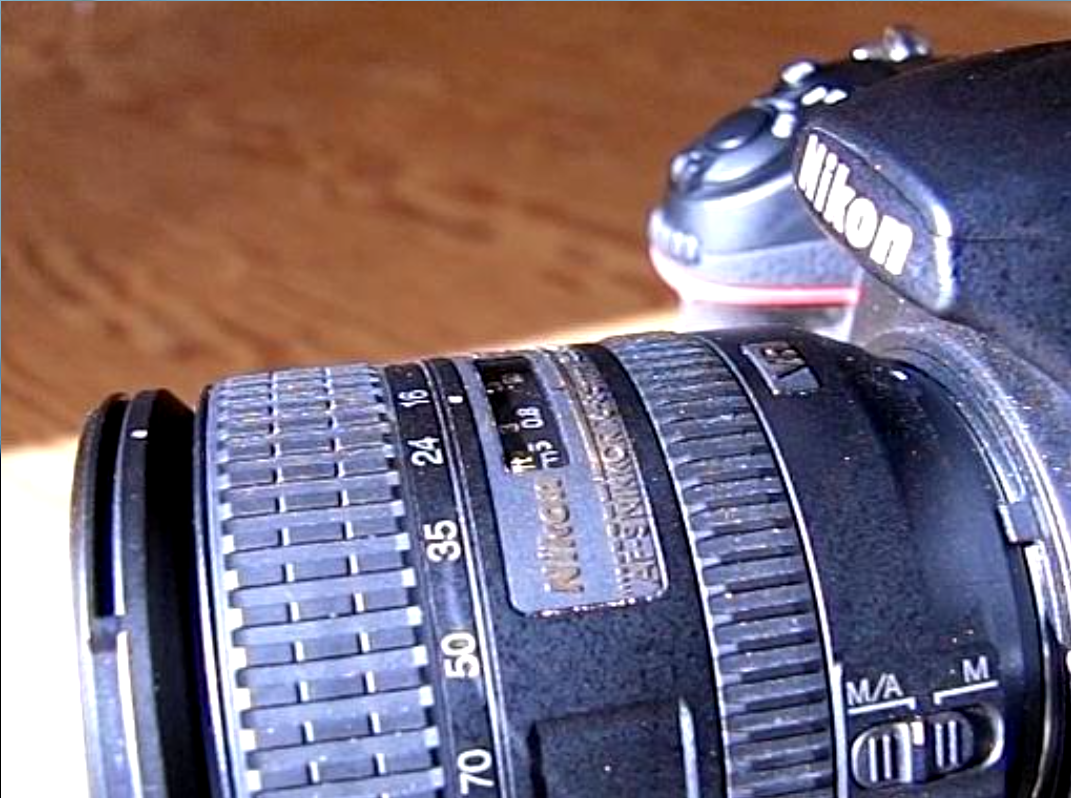
\includegraphics[height=2cm]{camera.png}}
    node[pos=0.8,sloped,draw=orange,inner sep=.1mm,opacity=0]
      {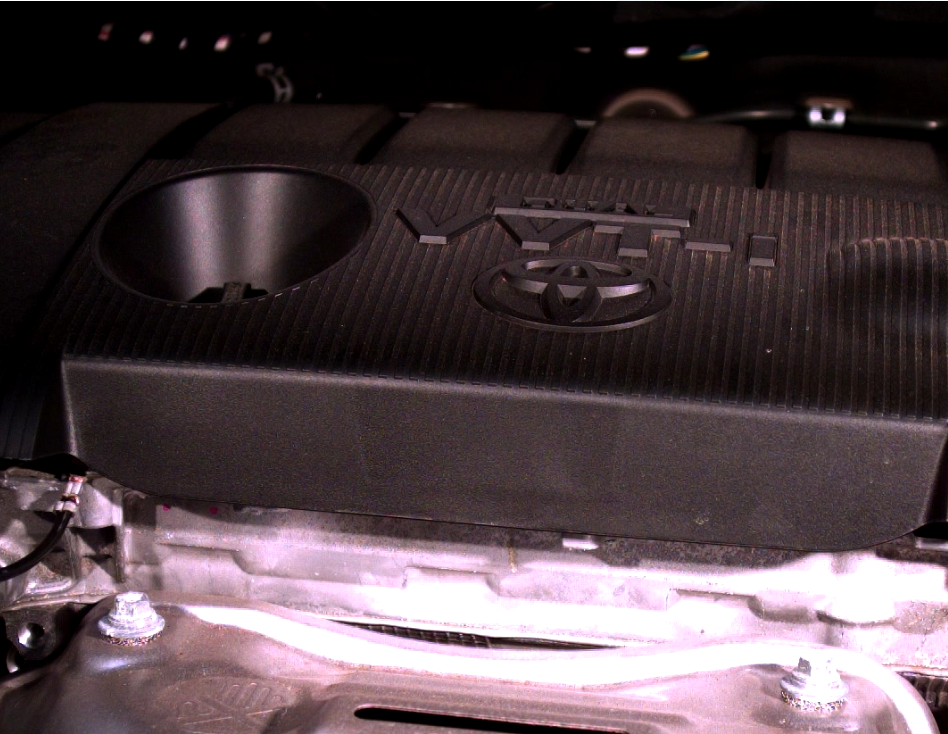
\includegraphics[height=2cm]{engine.png}}
    node[pos=1,sloped,draw=orange,inner sep=.1mm,opacity=0]
      {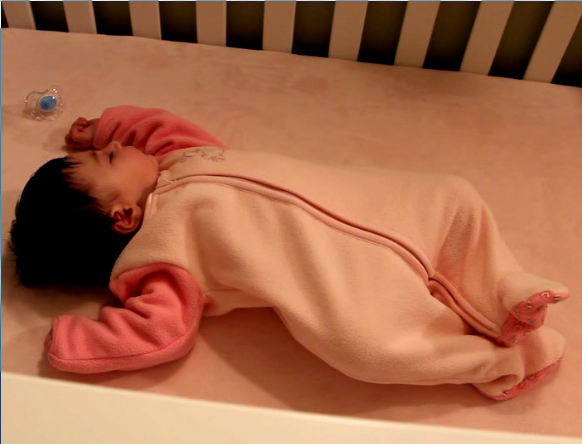
\includegraphics[height=2cm]{baby.png}};
    \end{tikzpicture}}
  \only<4>{
  \begin{tikzpicture}
    \draw[draw=white] (0,0) .. controls (3,1.3) and (6,1.3) .. (9,0)
    node[pos=0,sloped,draw=orange,inner sep=.1mm]
      {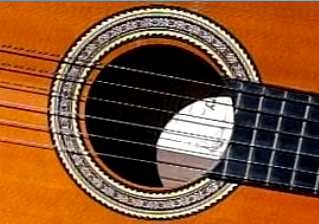
\includegraphics[height=2cm]{guitar.png}}
    node[pos=0.2,sloped,draw=orange,inner sep=.1mm]
      {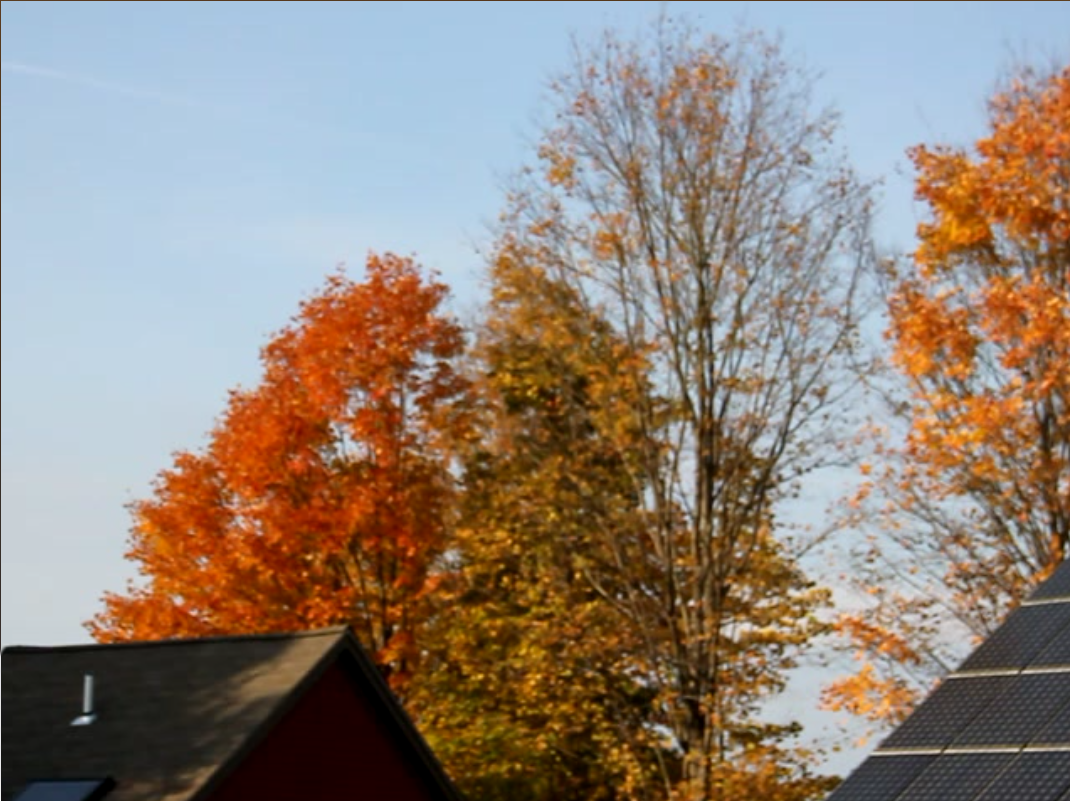
\includegraphics[height=2cm]{trees.png}}
    node[pos=0.4,sloped,draw=orange,inner sep=.1mm]
      {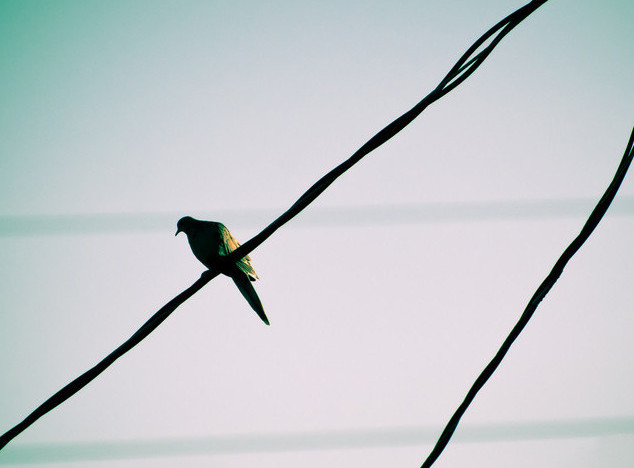
\includegraphics[height=2cm]{birds.jpg}}
    node[pos=0.6,sloped,draw=orange,inner sep=.1mm]
      {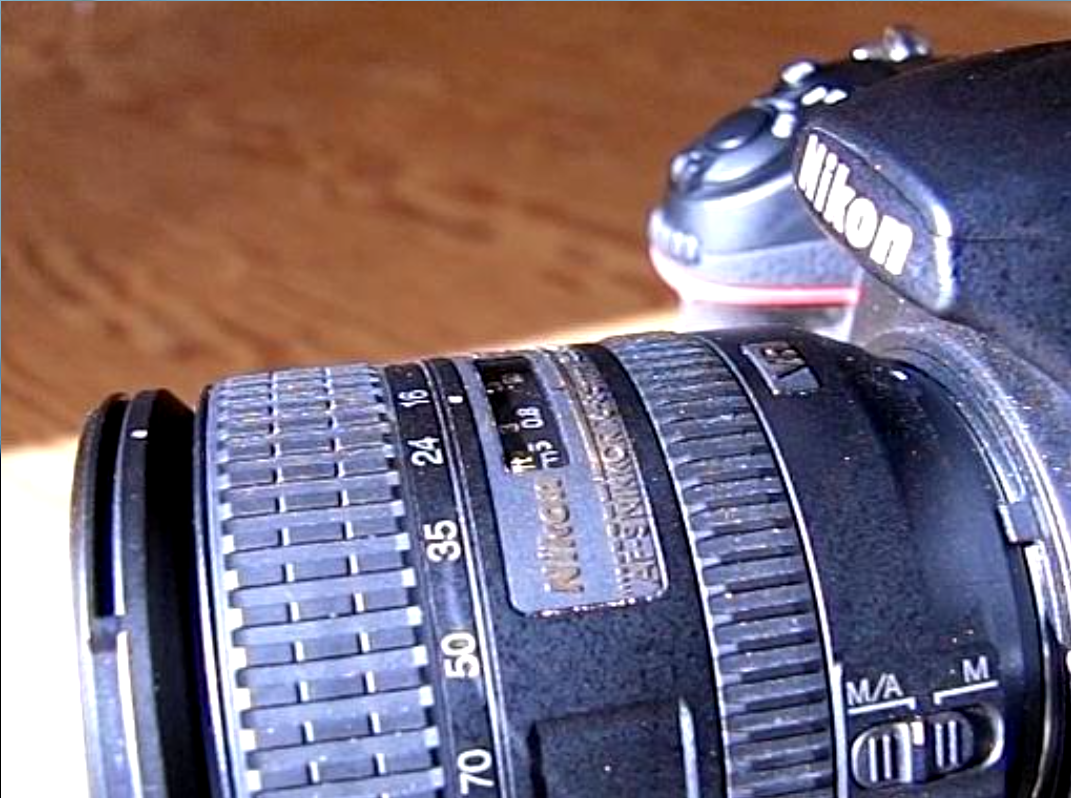
\includegraphics[height=2cm]{camera.png}}
    node[pos=0.8,sloped,draw=orange,inner sep=.1mm,opacity=0]
      {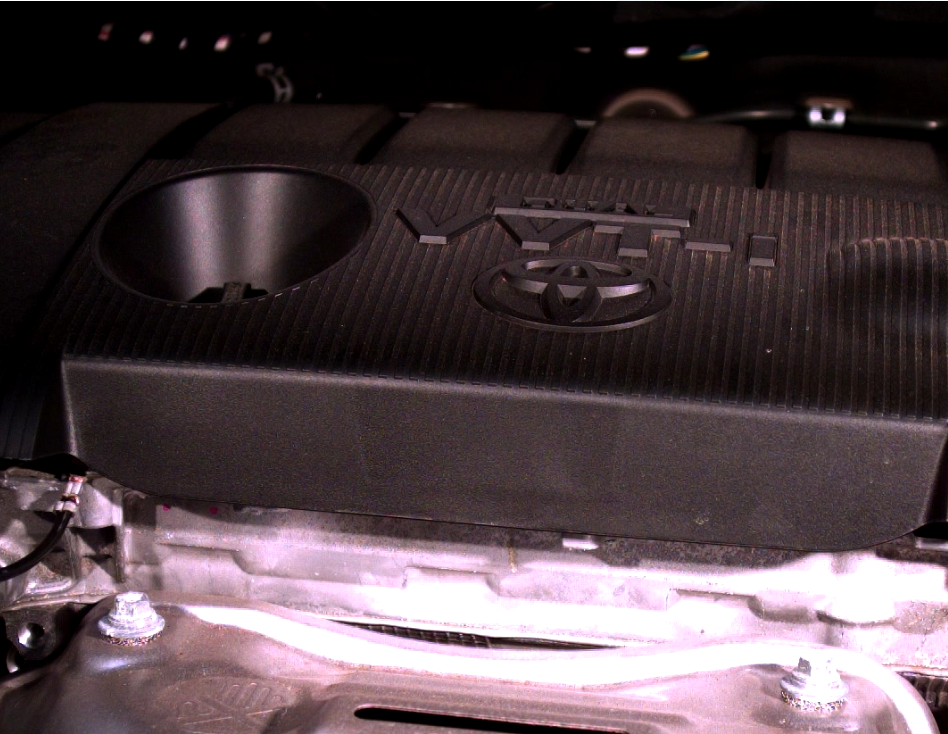
\includegraphics[height=2cm]{engine.png}}
    node[pos=1,sloped,draw=orange,inner sep=.1mm,opacity=0]
      {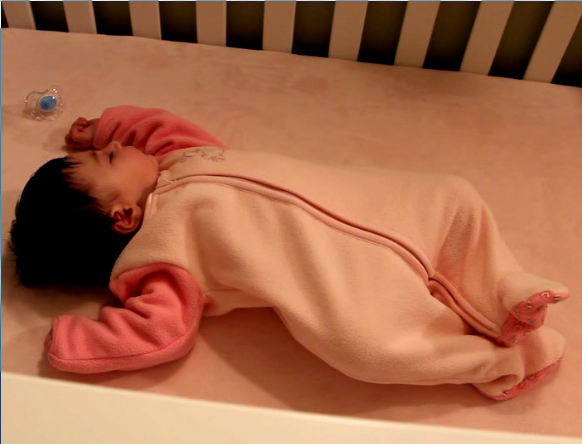
\includegraphics[height=2cm]{baby.png}};
    \end{tikzpicture}}
  \only<5>{
  \begin{tikzpicture}
    \draw[draw=white] (0,0) .. controls (3,1.3) and (6,1.3) .. (9,0)
    node[pos=0,sloped,draw=orange,inner sep=.1mm]
      {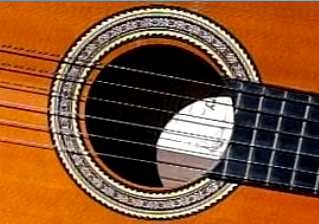
\includegraphics[height=2cm]{guitar.png}}
    node[pos=0.2,sloped,draw=orange,inner sep=.1mm]
      {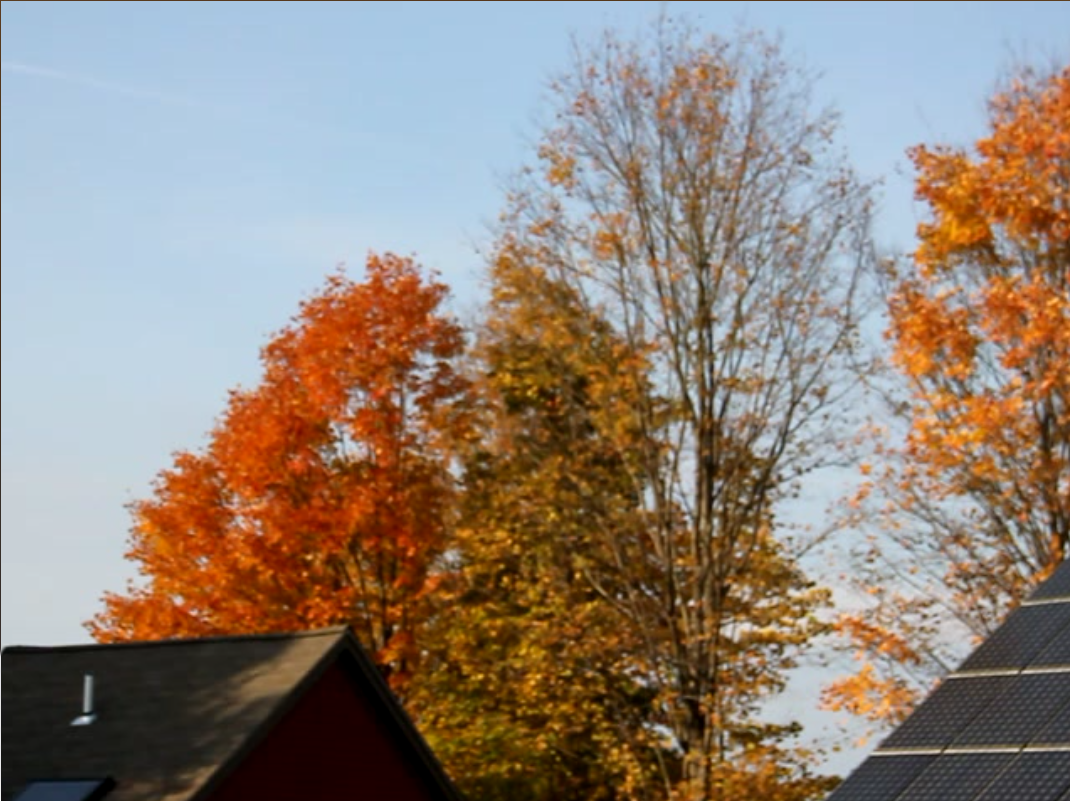
\includegraphics[height=2cm]{trees.png}}
    node[pos=0.4,sloped,draw=orange,inner sep=.1mm]
      {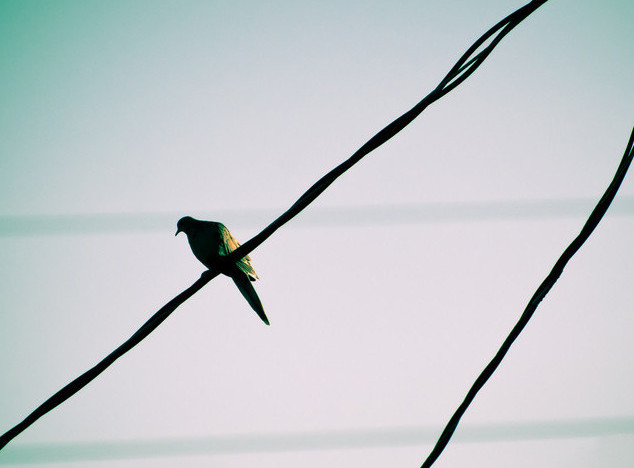
\includegraphics[height=2cm]{birds.jpg}}
    node[pos=0.6,sloped,draw=orange,inner sep=.1mm]
      {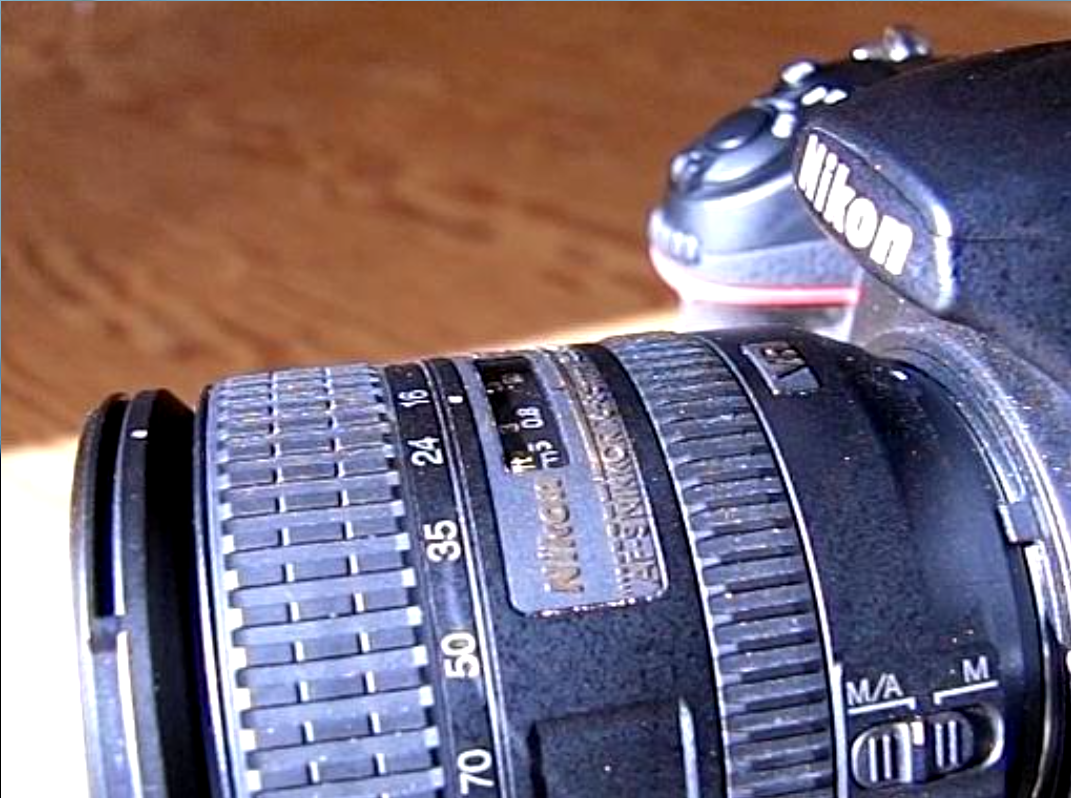
\includegraphics[height=2cm]{camera.png}}
    node[pos=0.8,sloped,draw=orange,inner sep=.1mm]
      {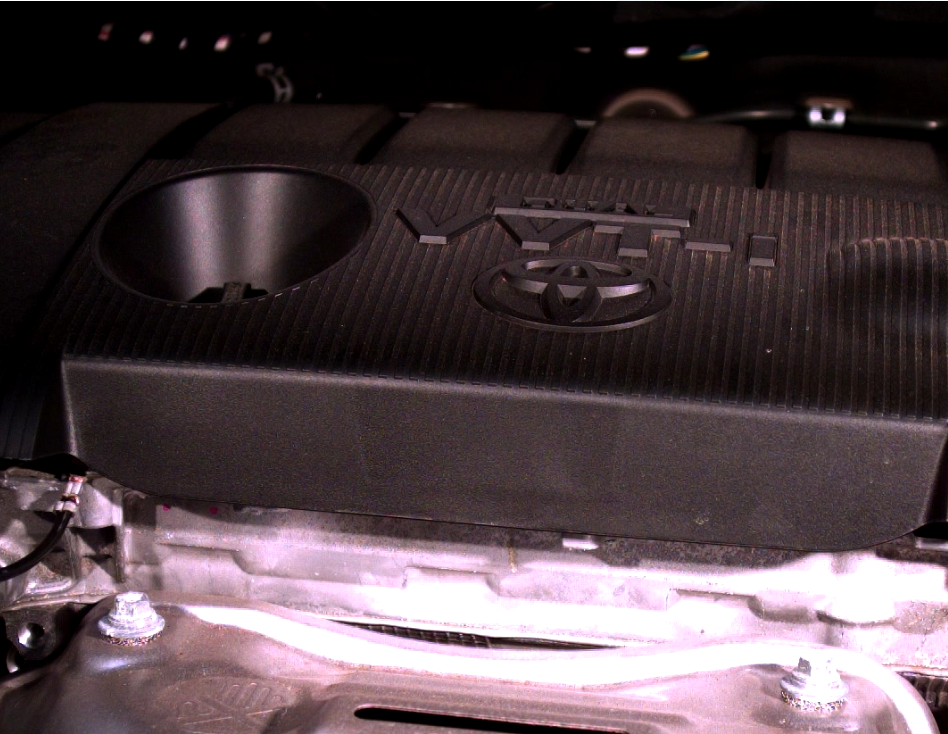
\includegraphics[height=2cm]{engine.png}}
    node[pos=1,sloped,draw=orange,inner sep=.1mm,opacity=0]
      {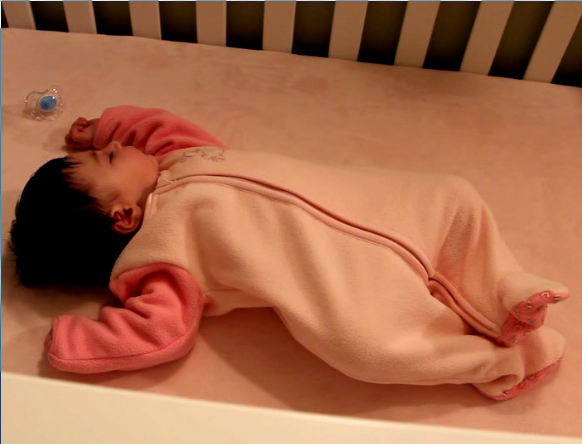
\includegraphics[height=2cm]{baby.png}};
    \end{tikzpicture}}
  \only<6>{
  \begin{tikzpicture}
    \draw[draw=white] (0,0) .. controls (3,1.3) and (6,1.3) .. (9,0)
    node[pos=0,sloped,draw=orange,inner sep=.1mm]
      {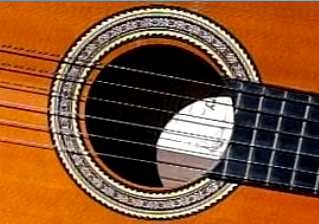
\includegraphics[height=2cm]{guitar.png}}
    node[pos=0.2,sloped,draw=orange,inner sep=.1mm]
      {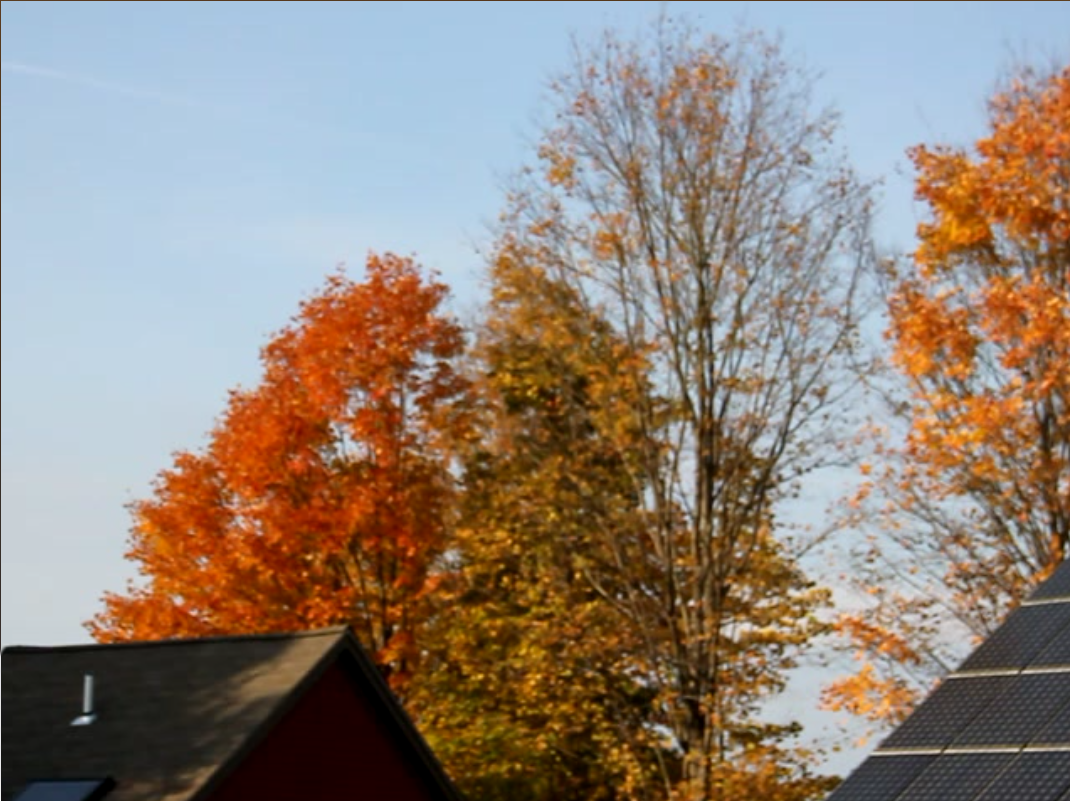
\includegraphics[height=2cm]{trees.png}}
    node[pos=0.4,sloped,draw=orange,inner sep=.1mm]
      {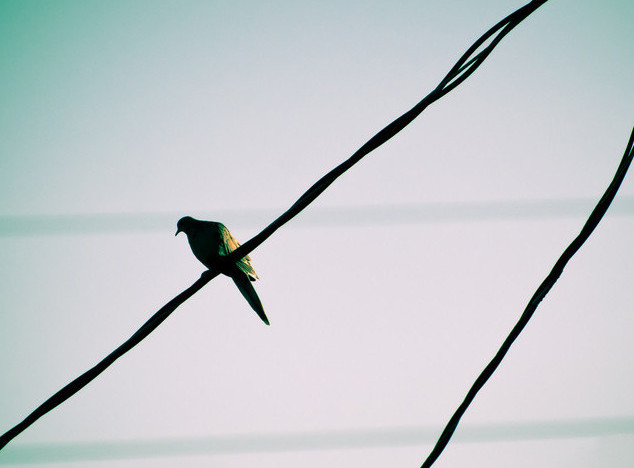
\includegraphics[height=2cm]{birds.jpg}}
    node[pos=0.6,sloped,draw=orange,inner sep=.1mm]
      {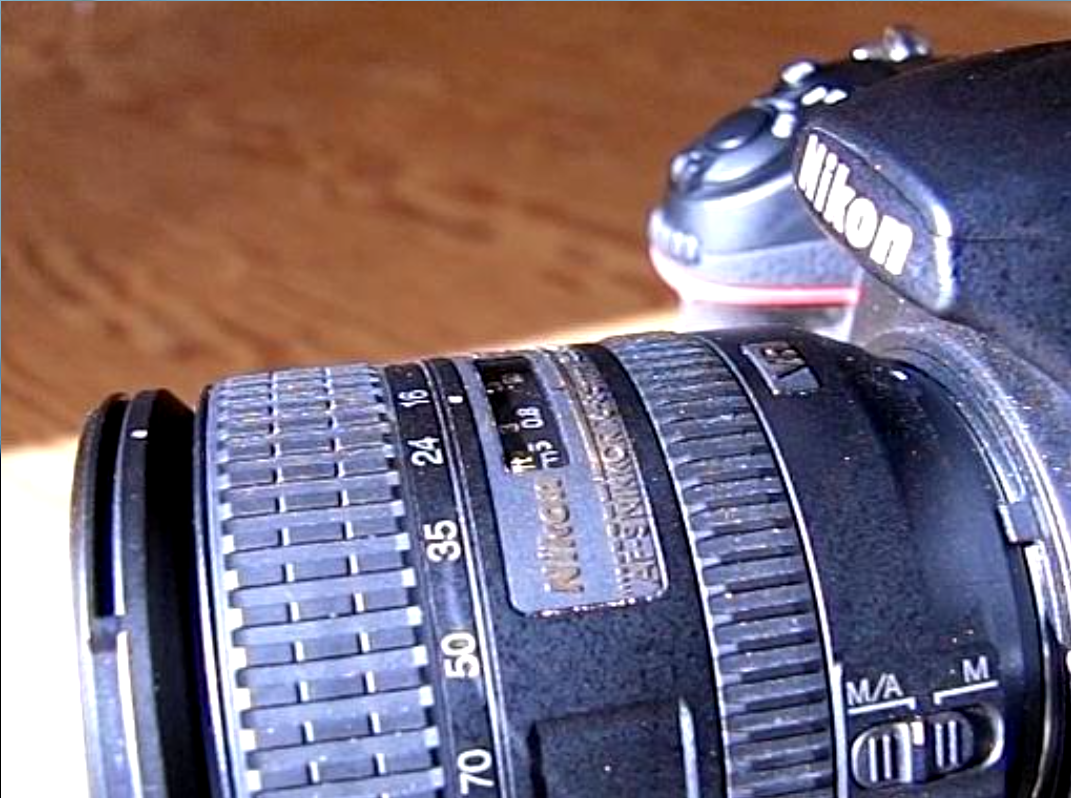
\includegraphics[height=2cm]{camera.png}}
    node[pos=0.8,sloped,draw=orange,inner sep=.1mm]
      {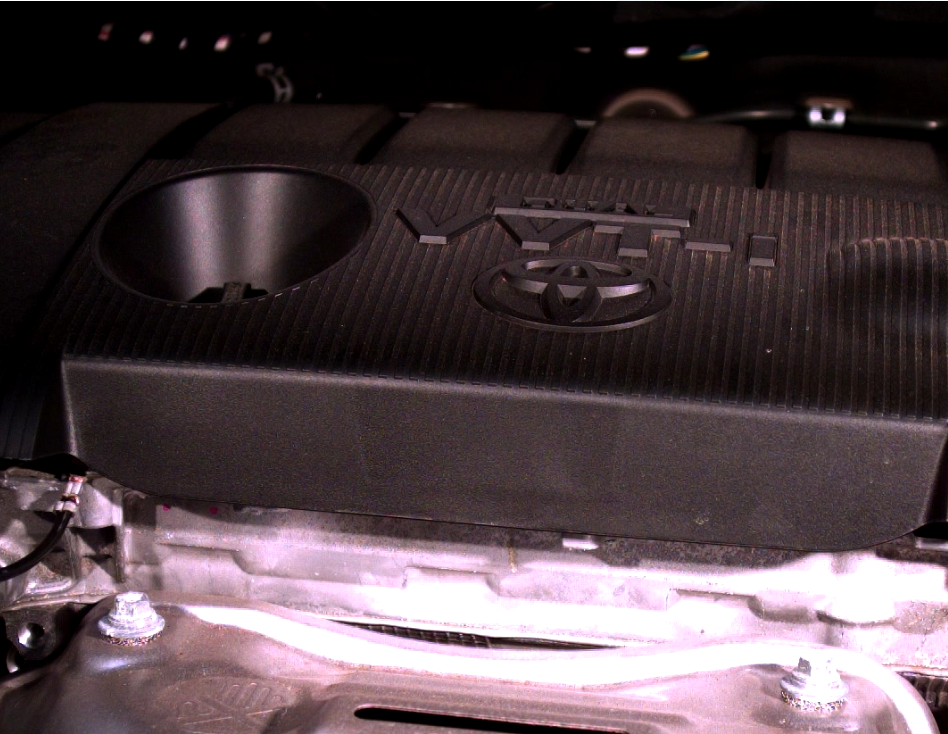
\includegraphics[height=2cm]{engine.png}}
    node[pos=1,sloped,draw=orange,inner sep=.1mm]
      {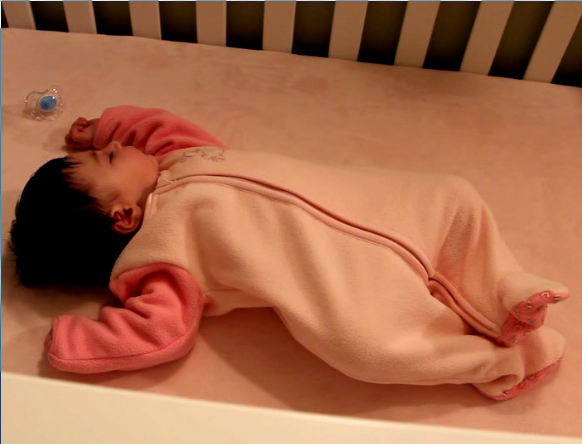
\includegraphics[height=2cm]{baby.png}};
    \end{tikzpicture}}
  \end{center}
  \only<6>{
  \begin{block}{}
    \begin{center}
      一花一世界,一叶一菩提。
    \end{center}
  \end{block}
  }
\end{frame}

\begin{frame}
  \frametitle{影像动作放大技术}
  影像动作放大技术是一种用于改变影像中感兴趣信号的变化幅度的技术。这类技术可以将
  生活中原本裸眼无法感知的微弱变化放大到裸眼可以感知的幅度,从而挖掘出有价值的信
  息。

  \medskip

  现有的方法:
  \begin{itemize}
  \item 拉格朗日视角的方法:\cite{liu2005motion};
  \item 欧拉视角的方法:\cite{wu2012eulerian, Wadhwa2013PhaseBased}。
  \end{itemize}
\end{frame}

\begin{frame}
  \frametitle{拉格朗日视角和欧拉视角}
  \small
  拉格朗日视角和欧拉视角是流体动力学中研究流场的两种视角。\pause

  \begin{itemize}
  \item 拉格朗日视角:通过观察场景中一些独立的粒子在时空中的运动轨迹来分析流体的
    运动。\pause
  \item 欧拉视角:通过观察流体在一些特定时刻的运动情况来分析流体的运动。
  \end{itemize}

  \medskip
  \only<1>{\vspace{1.95cm}}
  \begin{columns}
    \centering
    \begin{column}{0.2\textwidth}
      \only<2,3>{\fbox{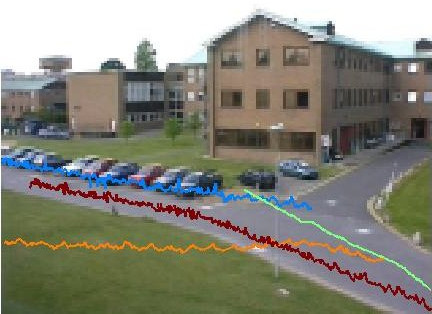
\includegraphics[height=2.2cm]{trajectories.jpg}}}
    \end{column}
    \begin{column}{0.6\textwidth}
      \only<3>{\fbox{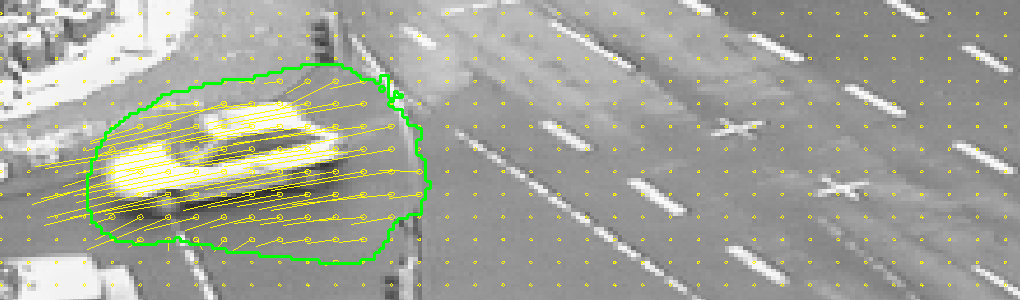
\includegraphics[height=2.2cm]{car-tracking2.jpg}}}
    \end{column}
  \end{columns}
\end{frame}

\begin{frame}
  \frametitle{拉格朗日视角的动作放大技术}
  2005年,文献 \cite{liu2005motion} 提出了一种拉格朗日视角的影像动作放大方法。

  \medskip
  
  \begin{columns}
    \tiny
    \column{.3\textwidth}
    \centering
    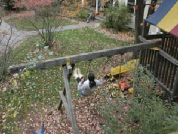
\includegraphics[width=\textwidth]{lag1.png}\\
    视频校准
    \column{.3\textwidth}
    \centering
    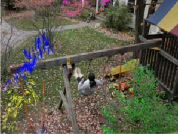
\includegraphics[width=\textwidth]{lag2.png}\\
    特征点轨迹聚类
    \column{.3\textwidth}
    \centering
    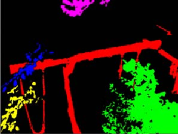
\includegraphics[width=\textwidth]{lag3.png}\\
    分割动作层
  \end{columns}

  \medskip
  \begin{columns}
    \tiny
    \column{.3\textwidth}
    \centering
    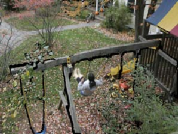
\includegraphics[width=\textwidth]{lag4.png}\\
    直接放大结果(出现了空洞)
    \column{.3\textwidth}
    \centering
    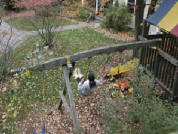
\includegraphics[width=\textwidth]{lag5.png}\\
    进行背景填充得到的结果
    \column{.3\textwidth}
    \centering
    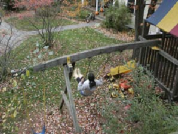
\includegraphics[width=\textwidth]{lag6.png}\\
    先对动作层进行人工编辑再放大的结果
  \end{columns}
\end{frame}

\begin{frame}
  \frametitle{拉格朗日视角的动作放大技术 --- 结果示例}
  \begin{figure}[htbp]
    \centering
    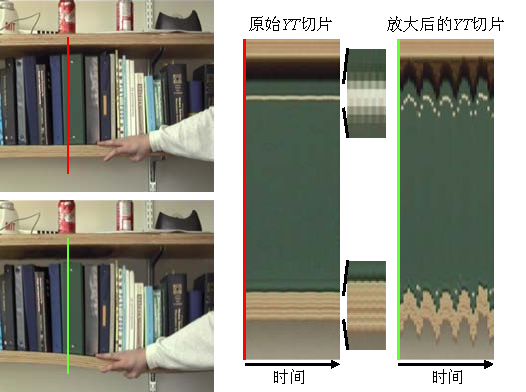
\includegraphics[width=.7\textwidth]{liu.pdf}
    \label{fig:liu}
  \end{figure}
\end{frame}

\begin{frame}
  \frametitle{欧拉视角的动作放大技术 --- 线性方法}
  欧拉视角的影像动作放大方法又被称为欧拉影像放大技术(Eulerian Video
  Magnification, EVM)。2012 年,文献 \cite{wu2012eulerian} 提出了一种线性的欧拉
  影像动作放大方法。
  \begin{figure}[htbp]
    \centering
    \includegraphics[width=.9\textwidth]{linear.pdf}
    \label{fig:linear}
  \end{figure}
\end{frame}

\begin{frame}
  \frametitle{欧拉视角的动作放大技术 --- 结果示例}
  \small
  与拉格朗日视角的方法相比,欧拉视角的动作放大方法运算速度快,无需对放大后的结果进
行背景填充。除此之外,该方法不仅可以用来放大动作的变化,还可以用来放大颜色的变化。
  \begin{figure}[htbp]
  \centering
    \includegraphics[width=.65\textwidth]{motion-color-1.pdf}\\
    \includegraphics[width=.65\textwidth]{motion-color-2.pdf}\\
    \includegraphics[width=.65\textwidth]{motion-color-3.pdf}\\
  \end{figure}
\end{frame}

\begin{frame}
  \frametitle{欧拉视角的动作放大技术 --- 基于相位的方法}
  \small
  
  线性的欧拉影像动作放大方法会在放大动作的同时放大噪声,所允许的放大倍数也较
  小。2013年,文献\cite{Wadhwa2013PhaseBased}提出了一种基于相位的改进算法。基于相
  位的欧拉影像放大技术在放大动作的同时不会放大噪声,而是平移了噪声,因此允许更大
  的放大倍数。

  \begin{figure}[htbp]
  \centering
  \includegraphics[width=.9\textwidth]{phase.pdf}
  \label{fig:phase-based}
  \end{figure}
\end{frame}

\begin{frame}
  \frametitle{欧拉视角的动作放大技术 --- 结果对比}
  线性的方法和基于相位的方法的结果对比:

  \begin{figure}[htbp]
  \centering
  \includegraphics[width=\textwidth]{compare.pdf}
  \label{fig:compare}
\end{figure}
\end{frame}

\begin{frame}
  \frametitle{欧拉视角的动作放大技术 --- “鬼影”问题}

  \small
  
  对于存在大幅度动作的场景,直接使用现有的欧拉影像动作放大技术会产生明显的“鬼
  影”现象,从而影响放大效果。

  \medskip

  \begin{columns}
    \small
    \column{.5\textwidth}
    \centering
    \includegraphics[width=.9\textwidth]{ghost-linear.png}\\
    线性的方法
    \column{.5\textwidth}
    \centering
    \includegraphics[width=.9\textwidth]{ghost-phase.png}\\
    基于相位的方法
  \end{columns}

  \medskip
  
  此外,对场景中的非感兴趣区域的放大也会影响对放大结果的后继分析,如心率提取等。
\end{frame}

\begin{frame}
  \frametitle{欧拉视角的动作放大技术 --- “鬼影”问题}
  \small
  
  对于这个问题,文献\cite{Wadhwa2013PhaseBased}将相位的变化幅度超过一个阈值的动作
  的放大倍数都设为0来避免对这些区域进行放大。然而,这个方法直接忽略了存在大幅度动
  作的物体,因而无法对大幅度动作中的物体的细节变化进行放大。

  \medskip
  \begin{columns}
    \small
    \column{.5\textwidth}
    \raggedleft
    \begin{minipage}{0.7\textwidth}
      \centering
      \includegraphics[width=\textwidth]{ignore.pdf}\\
      直接全局放大结果
    \end{minipage}
    \column{.5\textwidth}
    \begin{minipage}{0.7\textwidth}
      \centering
      \includegraphics[width=\textwidth]{ignore2.pdf}\\
      忽略大幅度运动的物体
    \end{minipage}
  \end{columns}
\end{frame}

\section{本文工作}

\begin{frame}
  \frametitle{本文工作(What)}
  \vspace{-2.5em}
  \begin{figure}
    \centering
    \includegraphics[width=\textwidth, page=3]{mindmap.pdf}
  \end{figure}
\end{frame}

\begin{frame}
  \frametitle{本文工作(What)}
  \begin{itemize}[<+->]
  \item 提出了一种结合了拉格朗日视角和欧拉视角的优点的影像动作放大方法;
  \item 基于CIEL*a*b*颜色空间的颜色衰减;
  \item 基于四元数的理想带通滤波。
  \end{itemize}
\end{frame}

\section{算法细节}

\begin{frame}
  \frametitle{算法细节(How)}
  \vspace{-2.5em}
  \begin{figure}
    \centering
    \includegraphics[width=\textwidth, page=4]{mindmap.pdf}
  \end{figure}
\end{frame}

\begin{frame}
  \frametitle{算法框架图}
  \centering
  \scriptsize
    \only<1>{\includegraphics[width=\textwidth, page=1]{fc-evm.pdf}\\\medskip 读
      入视频}
    % \only<2>{\includegraphics[width=\textwidth, page=2]{fc-evm.pdf}}
    \only<2>{\includegraphics[width=\textwidth, page=3]{fc-evm.pdf}\\\medskip 选
      择感兴趣的区域}
    \only<3>{\includegraphics[width=\textwidth, page=4]{fc-evm.pdf}\\\medskip 区
      域跟踪,提取前景掩码}
    \only<4>{\includegraphics[width=\textwidth, page=5]{fc-evm.pdf}\\\medskip 空
      间滤波}
    \only<5>{\includegraphics[width=\textwidth, page=6]{fc-evm.pdf}\\\medskip 频
      域滤波}
    \only<6>{\includegraphics[width=\textwidth, page=7]{fc-evm.pdf}\\\medskip 放
      大和叠加}
    \only<7>{\includegraphics[width=\textwidth, page=8]{fc-evm.pdf}\\\medskip 基
      带混合}
    \only<8>{\includegraphics[width=\textwidth,
      page=9]{fc-evm.pdf}\\\medskip 重构图像}
    \only<9>{\includegraphics[width=\textwidth,
      page=10]{fc-evm.pdf}\\\medskip 合成并输出视频}
\end{frame}

\subsection{区域跟踪}

\begin{frame}
  \frametitle{区域跟踪}
  \vspace{-2.5em}
  \begin{figure}
    \centering
    \includegraphics[width=\textwidth, page=5]{mindmap.pdf}
  \end{figure}
\end{frame}

\begin{frame}
  \frametitle{区域跟踪}
  使用\cite{常发亮2007}提出的Mean-shift跟踪与Kalman滤波相结合的算法对视频中
  的每一帧进行区域跟踪。

  \begin{itemize}
  \item Mean-shift算法:一种在一组数据的密度分布中寻找局部极值的算法;
  \item Kalman滤波:又称为线性二次估计。能够从一系列的不完全的,包含噪声的测量中预测目标的运动位置和速度。
  \end{itemize}
\end{frame}

\iffalse
\begin{frame}
  \frametitle{Mean-shift 算法 --- 模式计算}
  \begin{block}{目标模式}
    首先将图像由RGB色彩空间转换到HSV色彩空间,提取出Hue分量,并将其分成$m$等
    份,每一等份对应一个子特征值,则第$u$个特征值的概率分布
    为\cite{duda1973pattern}:
\begin{equation}
  \label{eq:characteristic-prob}
  q_{u}=C\sum_{i=1}^{n}k\left( \left\| \frac{x_{0}-x_{i}}{h} \right\|^{2}
  \right)\delta[b(x_{i})-u],\qquad i\in[1,\ldots,n]
\end{equation}
\end{block}

\pause

\begin{block}{目标候选模式}
  假设$y_0$是当前帧的目标候选区域的中心点,则其概率分布为:
\begin{equation}
  \label{eq:target-candidate}
  p_{u}(y_0)=C\sum_{i=1}^{n}k\left( \left\| \frac{y_{0}-x_{i}}{h} \right\|^{2}
  \right)\delta[b(x_{i})-u],\qquad i\in[1,\ldots,n]
\end{equation}
\end{block}
\end{frame}

\begin{frame}
  \frametitle{Mean-shift 算法 --- 相似度衡量}
  \begin{block}{相似度衡量}
    引入Bhattacharyya系数来衡量目标模式与目标候选模式的相似度:
\begin{equation}
  \label{eq:Bhattacharyya}
  \rho(\rho(y),q)=\sum_{u=1}^{m}\sqrt{p_{u}(y)q_{u}}
\end{equation}

对于两个颜色分布直方图的匹配,可以定义如下的距离公式,计算两个分布之间的距离:
\begin{equation}
  \label{eq:distance}
  d(y)=\sqrt{1-\rho(y)}
\end{equation}
$d(y)$ 越小,两个颜色分布直方图越相近。
  \end{block}
\end{frame}

\begin{frame}
  \frametitle{Mean-shift 算法 --- 搜索策略}
  \small
  在搜索阶段,算法使用梯度下降的策略搜索使Bhattacharyya系数达到最大的目标候选区
  域。
  
    对$\rho(\rho(y),q)$进行泰勒级数展开可得:
\begin{equation}
  \label{eq:taylor}
  \rho(\rho(y),q)\approx \frac{1}{2}\sum_{u=1}^{m}\sqrt{p_u(y_0)q_u}+\textcolor{red}{\frac{C}{2}\sum_{u=1}^{m}w_{i}k(\left\|y-x_i\right\|^2)}
\end{equation}

其中,
\begin{equation}
    \label{eq:weight}
    w_{i}=\sum_{i=1}^{m}\sqrt{\frac{q_u}{p_{u}(y_0)}}\delta[b(x)-u]
\end{equation}

要使Bhattacharyya系数最大,即是使公式\ref{eq:taylor}的\textcolor{red}{第二项}达到最大。
因此,可沿梯度方向确定下一个目标候选区域的位置:
    \begin{equation}
    \label{eq:next-position}
    y_{i}=\frac{\sum_{i=1}^{m}x_{i}w_{i}g\left(\left\|\frac{y_0-x_i}{h}\right\|^{2}\right)}{\sum_{i=1}^{m}w_{i}g\left(\left\|\frac{y_0-x_i}{h}\right\|^{2}\right)}
  \end{equation}
\end{frame}

\begin{frame}
  \frametitle{Mean-shift 算法 --- 搜索过程}
  \begin{exampleblock}{Mean-shift搜索算法}
    \textcolor{black!60!green}{输入}: 目标模式$q_u$及上一帧的目标窗口的位置$y_0$ 。\vspace{-.5em}
    \begin{enumerate}[(S1)]
    \item 初始化当前帧的搜索窗口为$y_0$,根据公
    式\ref{eq:target-candidate}计算$p_u(y_0)$,根据公式
   \ref{eq:Bhattacharyya}评估$\rho(\rho(y_0),q)$。
    \item 根据公式\ref{eq:weight}计算每一点的权值$w_{i}$ 。
    \item 根据公式\ref{eq:next-position}计算下一个目标候选区域的位置$y_{i}$
   。
    \item 根据公式\ref{eq:target-candidate}计算$p_u(y_1)$ ,根据公式
   \ref{eq:Bhattacharyya}评估$\rho(\rho(y_1),q)$。
    \item 如果$\left\|y_{i}-y_{0}\right\|$小于一个目标值$\varepsilon$,或者
    迭代次数超过了预先设定的最大迭代次数,则结束迭代;\\
    否则,令$y_{0}\leftarrow y_{i}$,返回步骤 2。
    \end{enumerate}
  \end{exampleblock}
\end{frame}

\begin{frame}[allowframebreaks]
  \frametitle{Kalman滤波 --- 基本模型}
  \begin{block}{状态方程}
    \begin{equation}
    \label{eq:state}
    X_{k}=F\cdot X_{k-1}+W_k
  \end{equation}
\end{block}

\begin{block}{观测方程}
  \begin{equation}
    \label{eq:observation}
    Z_{k}=H\cdot X_{k}+K_{k}
  \end{equation}  
\end{block}

其中,$X_k = [x,y,dx,dy]^{T}$是系统在$k$时刻的状态向量,$x$和$dx$分别是水平
方向的位置和速度,$y$和$dy$则分别是竖直方向的位置和速度。$Z_k=[x,y]^{T}$是
系统在$k$时刻的观测向量,表示观测目标的位置。$W_k$和$V_k$分别为状态和观测对
应的高斯噪声向量,其方差矩阵分别为$Q$和$R$。$F$为状态转移矩阵,$H$为观测矩阵。

四个矩阵的值分别为\cite{Zhang2009}:$$F=\begin{bmatrix}
  1 & 0 & 1 & 0\\0 & 1 & 0 & 1 \\ 0 & 0 & 1 & 0\\ 0 & 0 & 0 & 1
\end{bmatrix}
\mbox{,}~
H = \begin{bmatrix}
  1 & 0 & 0 & 0\\0 & 1 & 0 & 0
\end{bmatrix}
\mbox{,}~
Q=\begin{bmatrix}
  1 & 0 & 0 & 0\\0 & 1 & 0 & 0 \\ 0 & 0 & 1 & 0\\ 0 & 0 & 0 & 1
\end{bmatrix}
\mbox{,}~
R = \begin{bmatrix}
  1 & 0 \\0 & 1 
\end{bmatrix}
$$
\end{frame}

\begin{frame}
  \frametitle{Kalman滤波 --- 算法}
  \begin{exampleblock}{Kalman滤波}
    \scriptsize
    \begin{enumerate}[(S1)]
    \item 初始化:
    \begin{eqnarray*}
      \hat{X}_0&=&E[X_0]\\
      P_0&=&E[(X_0-E[X_0])(X_0-E[X_0])^{T}]
    \end{eqnarray*}
    \item 预测:
    \begin{eqnarray*}
      \hat{X}_{k+1,k}&=&F \hat{X}_{k}\\ 
      P_{k+1,k}&=&F P_{k}F^{T}+Q\\
      K_{k+1}&=&P_{k+1,k}H^{T}(H P_{k+1,k}H^{T}+R)^{-1}
    \end{eqnarray*}
    \item 估计:
    \begin{eqnarray*}
      \hat{X}_{k+1}&=&\hat{X}_{k+1,k}+K(Z_{k+1}-H\hat{X}_{k+1,k})\\
      P_{k+1}&=&(I-K_{k+1}H)P_{k+1,k}
    \end{eqnarray*}
    \end{enumerate}
  \end{exampleblock}
\end{frame}
\fi

\begin{frame}[t]
  \frametitle{Mean-shift与Kalman滤波相结合的跟踪算法}
  $k+1$时刻目标的位置$\hat{X}_{k+1}$:

  \medskip
  \begin{beamercolorbox}[shadow=true,sep=0pt,rounded=true]{box}
    \begin{equation}
      \label{eq:target-pos}
      \hat{X}_{k+1}={\color<4>{blue}\sigma}{\color<3>{blue}\hat{X}_{k+1,k}}+(1-{\color<4>{blue}\sigma}){\color<2>{blue}y_1}
    \end{equation}
  \end{beamercolorbox}

  \medskip
  \begin{center}
  \setlength{\extrarowheight}{1.5mm}
  %\addtolength{\tabcolsep}{1mm}
  \rowcolors[]{1}{orange!70}{white!90!gray}
  \begin{tabular}{cl}
    \onslide<2->{$\color<2>{blue}y_1$}       & \onslide<2->{Mean-shift跟踪得到的目标位置}\\
    \onslide<3->{$\color<3>{blue}\hat{X}_{k+1,k}$} & \onslide<3->{由Kalman滤波预测的目标位置} \\
    \onslide<4->{$\color<4>{blue}\sigma$}         & \onslide<4->{比例因子,($0 \le \sigma \le 1$)}\\
  \end{tabular}
\end{center}

\end{frame}

\begin{frame}
  \frametitle{Mean-shift与Kalman滤波相结合的跟踪算法}
  \begin{block}{Bhattacharyya系数}
    \begin{equation}
      \label{eq:Bhattacharyya}
      \rho(\rho(y),q)=\sum_{u=1}^{m}\sqrt{p_{u}(y)q_{u}}
    \end{equation}
  \end{block}

  \pause
  \begin{exampleblock}{Mean-shift和Kalman滤波相结合的跟踪算法}
  \begin{enumerate}[(S1)]
  \item 初始化目标的位置和速度;
  \item 使用Kalman预测目标在当前帧的位置$\hat{X}_{k+1,k}$;
  \item 使用Mean-shift算法获得目标在当前帧的位置$y_1$;
  \item 根据公式 \ref{eq:Bhattacharyya} 计算Bhattacharyya系数的值,选择合适的
    $\sigma$值,再根据公式 \ref{eq:target-pos} 计算目标位置$\hat{X}_{k+1}$ 。
  \end{enumerate}
\end{exampleblock}
  
\end{frame}

\subsection{前景分割}

\begin{frame}
  \frametitle{前景分割}
  \vspace{-2.5em}
  \begin{figure}
    \centering
    \includegraphics[width=\textwidth, page=6]{mindmap.pdf}
  \end{figure}
\end{frame}

\begin{frame}
  \frametitle{前景分割 --- 边界问题}

  如果直接对跟踪得到的区域图像序列进行欧拉影像动作放大,会导致最后的合成结果在区
  域边缘出现明显的边界。

  \begin{figure}[htbp]
    \centering
    \includegraphics[width=.5\textwidth]{bound-artifact.png}
  \end{figure}
\end{frame}

\begin{frame}
  \frametitle{前景分割 --- GrabCut 算法}
  GrabCut算法\cite{Rother2004}是在Graph Cuts算法\cite{Boykov2001}的基础上发展而来的一种简单直观的分割算法。
  \begin{figure}
    \centering
    \includegraphics[width=.6\textwidth]{grabcut.pdf}
  \end{figure}
\end{frame}

\begin{frame}
  \frametitle{前景分割 --- 分割过程}
  \scriptsize
  \centering
  \begin{columns}
    \column{.5\textwidth}
    \raggedleft
    \begin{minipage}{.7\linewidth}
      \centering
      \includegraphics[width=\textwidth]{grabcut-original.png}\\
      原视频帧
    \end{minipage}
    \column{.5\textwidth}
    \begin{minipage}{0.7\linewidth}
      \centering
      \includegraphics[width=\textwidth]{grabcut-track.png}\\
      区域跟踪结果
    \end{minipage}
  \end{columns}

  \medskip
  
  \begin{columns}
    \column{.5\textwidth}
    \raggedleft
    \begin{minipage}{0.7\linewidth}
      \centering
      \includegraphics[width=\textwidth]{grabcut-mask.png}\\
      使用GrabCut提取得到的前景掩码
    \end{minipage}
    \column{.5\textwidth}
    \begin{minipage}{0.7\linewidth}
      \centering
      \includegraphics[width=\textwidth]{grabcut-roi.png}\\
      截取结果
    \end{minipage}
  \end{columns}
\end{frame}

\subsection{局部欧拉影像动作放大}

\begin{frame}
  \frametitle{局部欧拉影像动作放大}
  \vspace{-2.5em}
  \begin{figure}
    \centering
    \includegraphics[width=\textwidth, page=7]{mindmap.pdf}
  \end{figure}
\end{frame}

\begin{frame}
  \frametitle{基于CIEL*a*b*空间的颜色衰减 --- 原理}
  \begin{itemize}
  \item \cite{wu2012eulerian}、\cite{Wadhwa2013PhaseBased}:基于YIQ颜色空间的颜
    色衰减;
  \item 本文:基于CIEL*a*b*颜色空间的颜色衰减。
  \end{itemize}

  \begin{figure}[htbp]
  \scriptsize
  \centering
  \includegraphics[width=.5\textwidth]{color-plate.pdf}\\
  CIEL*a*b*颜色空间模型图
  \end{figure}
\end{frame}

\begin{frame}
  \frametitle{基于CIEL*a*b*空间的颜色衰减 --- 结果}
  \small
  将图像由RGB颜色空间转为CIEL*a*b*颜色空间并对图像进行动作放大后,引入一个衰减因
  子\alert{$\mu$}($0\le \mu \le 1$)衰减I、Q两个通道的变化。

  \begin{center}
    \includegraphics[width=.8\textwidth]{attenuation-before.png}\\
    衰减前,图像存在较多颜色噪点\\
  \end{center}
\end{frame}

\begin{frame}
  \frametitle{基于CIEL*a*b*空间的颜色衰减 --- 结果}
  \small
  将图像由RGB颜色空间转为CIEL*a*b*颜色空间并对图像进行动作放大后,引入一个衰减因
  子\alert{$\mu$}($0\le \mu \le 1$)衰减I、Q两个通道的变化。

  \begin{center}
    \includegraphics[width=.8\textwidth]{attenuation-after.png}\\
    衰减后,颜色噪点被消除
  \end{center}
\end{frame}

\begin{frame}
  \frametitle{带通滤波 --- 带通滤波器的选择}
  \scriptsize
  \begin{itemize}
  \item 需要对放大结果进行后续的时频分析 --- 理想带通滤波器;
  \item 不需要进行后续的时频分析 --- 宽通带的带通滤波器(二级IIR带通滤波器、巴特沃斯带通滤波器)。
  \end{itemize}
  \tiny
  \begin{table}[htbp]
  \centering
  \label{tab:filters}
  \begin{tabular}[c]{cccc}
    \toprule[1.5pt]
    案例名称 & 代表帧 & 滤波器示意图 \\
    \midrule
    face & \mgape{\includegraphics[height=1cm]{face.jpg}}
    & \mgape{\includegraphics[height=1cm]{filter-face.pdf}} \\
    
    guitar & \mgape{\includegraphics[height=.85cm]{guitar.jpg}} &
    \mgape{\includegraphics[height=1cm]{filter-guitar.pdf}}\\
    subway & \mgape{\includegraphics[height=1cm]{subway.jpg}} & 
    \mgape{\includegraphics[height=1cm]{filter-subway.pdf}}\\
    wrist & \mgape{\includegraphics[height=1cm]{wrist.jpg}} &
    \mgape{\includegraphics[height=1cm]{filter-wrist.pdf}}
    \\
    \bottomrule[1.5pt]
  \end{tabular}
\end{table}
\end{frame}

\begin{frame}
  \frametitle{理想带通滤波 --- DFT}
  对一幅灰度图像进行频率域的理想带通滤波前,需要先对图像进行傅里叶变换,将其转换到
  频率域,再构造一个滤波器与之做乘积。二维数字图像的傅里叶变换(DFT)定义为:

  \medskip
  \begin{beamercolorbox}[shadow=true,sep=0pt,rounded=true]{box}
    \begin{equation}
      \label{eq:dft}
      F(u,v)=\sum_{x=0}^{M-1}\sum_{y=0}^{N-1}f(x,y)e^{-j2\pi(ux/M+vy/N)}
    \end{equation}
  \end{beamercolorbox}
  
  其中,离散变量$u$,$v$满足$u=0,1,2,\ldots,M-1$,$v=0,1,2,\ldots,N-1$。
\end{frame}

\begin{frame}
  \frametitle{理想带通滤波 --- 滤波步骤}
  \scriptsize
  \begin{exampleblock}{理想带通滤波器滤波步骤}
    \textcolor{black!60!green}{输入}: 大小为$M\times N$的彩色图像$f(x,y)$。\\
    \textcolor{black!60!green}{输出}: 滤波结果$g(x,y)$。\\ \vspace{-.5em}
    \begin{enumerate}[(S1)]
    \item 通道分解:将彩色图像$f(x,y)$分成三个通道的图像$f_1(x,y)$,
    $f_2(x,y)$和$f_3(x,y)$。
    \item 填充图像:对$f_i(x,y)$填充必要数量的0,形成大小为$P\times Q$的填充后的图像
    $f_{p}(x,y)$。
    \item 中心化图像:用$(-1)^{x,y}$乘以$f_{p}(x,y)$,使其移到变换的中心。
    \item DFT:根据公式\ref{eq:dft}计算来自步骤3的图像的DFT,得到$F(u,v)$。
    \item 理想带通滤波:$$G(u,v)=H(u,v)F(u,v)$$
    \item IDFT:$$g_p(x,y)=\left\{
      \mbox{real}[\Im^{-1}[G(u,v)]] \right\}(-1)^{x+y}$$ 
    \item 提取结果:从$g_p(x,y)$的左象限提取$M\times N$区域,得到该通道的滤波结
    果$g_i(x,y)$。
    \item 合并通道:将三个单通道的滤波结果重新合成一幅彩色图像$g(x,y)$。
    \end{enumerate}
  \end{exampleblock}
\end{frame}

\begin{frame}
  \frametitle{基于四元数的理想带通滤波 --- 四元数}
  将彩色图像的L*、a*、b*三个分量放入一个四元数\cite{hamilton1866elements}的矢量部
分,形成一个纯四元数。然后直接对其进行傅里叶变换和带通滤波等时频处理,具备更好的
整体性。

\medskip

\medskip
\begin{block}{四元数}
  一个四元数是如下形式的超复数:
  \begin{equation}
    \label{eq:quaternion}
    q=a+bi+cj+dk
  \end{equation}
  其中,$a$、$b$、$c$和$d$是实数,$i$、$j$和$k$是复数单位,且满足:
  \begin{equation}
  \label{eq:ijk}
  i^2=j^2=k^2=-1\mbox{,}ij=-ji=k\mbox{,}jk=-kj=i\mbox{,}ik=-ki=-j
\end{equation}
\end{block}
\end{frame}

\begin{frame}
  \frametitle{基于四元数的理想带通滤波 --- 四元数DFT}
  \cite{sangwine2000discrete}给出了一般性的四元数傅里叶变换:
  
  \medskip
\begin{beamercolorbox}[shadow=true,sep=0pt,rounded=true]{box}  
\begin{equation}
  \label{eq:quaternion-dft}
  F(u,v)=\frac{1}{\sqrt{MN}}\sum_{y=0}^{M-1}\sum_{x=0}^{N-1}e^{-\mu 2\pi((yv/M)+(xu/N))}f(x,y)
\end{equation}
\end{beamercolorbox}

  \medskip
在本文中,$f$是包含了L*,a*,b*三个分量的二维向量,即

  \medskip
\begin{beamercolorbox}[shadow=true,sep=0pt,rounded=true]{box}  
\begin{equation}
  \label{eq:quaternion-lab}
  f(x,y)=L^{*}(x,y)i+a^{*}(x,y)j+b^{*}(x,y)k
\end{equation}
\end{beamercolorbox}
\end{frame}

\begin{frame}
  \frametitle{基于四元数的理想带通滤波 --- 滤波步骤}
  \scriptsize
  \begin{exampleblock}{理想带通滤波器滤波步骤}
    \textcolor{black!60!green}{输入}: 大小为$M\times N$的四元数向量$f(x,y)$。\\
    \textcolor{black!60!green}{输出}: 滤波结果$g(x,y)$。\\ \vspace{-.5em}
    \begin{enumerate}[(S1)]
    \item 填充图像:对$f(x,y)$填充必要数量的0,形成大小为$P\times Q$的填充后的图像
    $f_{p}(x,y)$。
    \item 中心化图像:用$(-1)^{x,y}$乘以$f_{p}(x,y)$,使其移到变换的中心。
    \item DFT:根据公式\ref{eq:quaternion-dft}计算来自步骤3的图像的DFT,得到$F(u,v)$。
    \item 理想带通滤波:$$G(u,v)=H(u,v)F(u,v)$$
    \item IDFT:$$g_p(x,y)=\left\{
      \mbox{real}[\Im^{-1}[G(u,v)]] \right\}(-1)^{x+y}$$ 
    \item 提取结果:从$g_p(x,y)$的左象限提取$M\times N$区域,得到该通道的滤波结
    果$g(x,y)$。
    \end{enumerate}
  \end{exampleblock}
\end{frame}

\begin{frame}
  \frametitle{图像混合 --- 单基带混合}
  \small
  
  对每一层基带放大后,利用每一帧目标区域对应的前景掩码,将放大结果与原基带图像进
  行金字塔混合,将放大结果进一步约束在前景区域。
  
  \vspace{3em}

  \begin{columns}
    \begin{column}{.65\textwidth}
      \centering
      \fbox{\includegraphics[width=2.2cm]{apple.jpg}}~
      \fbox{\includegraphics[width=2.2cm]{mask.png}}~
      \fbox{\includegraphics[width=2.2cm]{orange.jpg}}
    \end{column}

    \begin{column}{.1\textwidth}
      \centering
      \Huge $\rightarrow$
    \end{column}
    
    \begin{column}{.2\textwidth}
      \centering
      \fbox{\includegraphics[width=2.2cm]{blend1.png}}
    \end{column}
  \end{columns}

  \medskip
  \centering {\scriptsize 单基带混合}
\end{frame}

\begin{frame}
  \frametitle{图像混合 --- 金字塔混合}
  本文采用多基带的金字塔混合方法\cite{ogden1985pyramid}。

  \medskip
  \begin{columns}
    \begin{column}{.65\textwidth}
      \centering
      \fbox{\scalebox{0.125}[0.125]{\includegraphics[width=2.2cm]{apple-level-3.png}}}~
      \fbox{\scalebox{0.125}[0.125]{\includegraphics[width=2.2cm]{mask.png}}}~
      \fbox{\scalebox{0.125}[0.125]{\includegraphics[width=2.2cm]{orange-level-3.png}}}\\
      \fbox{\scalebox{0.25}[0.25]{\includegraphics[width=2.2cm]{apple-level-2.png}}}~
      \fbox{\scalebox{0.25}[0.25]{\includegraphics[width=2.2cm]{mask.png}}}~
      \fbox{\scalebox{0.25}[0.25]{\includegraphics[width=2.2cm]{orange-level-2.png}}}\\
      \fbox{\scalebox{0.5}[0.5]{\includegraphics[width=2.2cm]{apple-level-1.png}}}~
      \fbox{\scalebox{0.5}[0.5]{\includegraphics[width=2.2cm]{mask.png}}}~
      \fbox{\scalebox{0.5}[0.5]{\includegraphics[width=2.2cm]{orange-level-1.png}}}\\
      \fbox{\includegraphics[width=2.2cm]{apple-level-0.png}}~
      \fbox{\includegraphics[width=2.2cm]{mask.png}}~
      \fbox{\includegraphics[width=2.2cm]{orange-level-0.png}}
    \end{column}

    \begin{column}{.1\textwidth}
      \centering
      \\
      {\Huge $\rightarrow$}
    \end{column}
    
    \begin{column}{.2\textwidth}
      \centering
      \fbox{\includegraphics[width=2.2cm]{blend2.png}}
    \end{column}
  \end{columns}

  \medskip
  \centering {\scriptsize 金字塔混合}
\end{frame}

\begin{frame}
  \frametitle{金字塔混合 --- 算法}
  \begin{exampleblock}{金字塔混合}
    \textcolor{black!60!green}{输入}: 大小相同的图像$A$,图像$B$及掩码图$M$。\\
    \textcolor{black!60!green}{输出}: 混合结果$C$。
    \begin{enumerate}[(S1)]
    \item 分别由图像$A$和图像$B$构造$n$层拉普拉斯金字塔$P_A$和$P_B$,
    由图像$M$构造$n$层高斯金字塔$P_M$。
    \item 对每一层基带,单独进行单基带混合,将混合结果存入一个新的拉普拉
    斯金字塔$P_C$的相同层。
    \item 根据$P_C$重建出图像$C$ 。
    \end{enumerate}
  \end{exampleblock}
\end{frame}

\begin{frame}
  \frametitle{金字塔混合 --- 结果}
  \scriptsize
  \begin{center}
    \includegraphics[width=.6\textwidth]{single-band-blend-asy.pdf}\\
    单基带混合,仍然可能存在边界

    \medskip
    \includegraphics[width=.6\textwidth]{pyramid-blend-asy.pdf}\\
    金字塔混合,边界问题得到改善
  \end{center}
\end{frame}

\section{实验结果}

\begin{frame}
  \frametitle{实验结果}
  \vspace{-2.5em}
  \begin{figure}
    \centering
    \includegraphics[width=\textwidth, page=8]{mindmap.pdf}
  \end{figure}
\end{frame}

\begin{frame}
  \frametitle{实验结果}
  \begin{figure}[htbp]
    \begin{tikzpicture}
      \draw[draw=white] (0,0) .. controls (3,1.3) and (6,1.3) .. (9,0)
      node[pos=0,sloped,draw=orange,inner sep=.1mm]
      {\includegraphics[height=2cm]{video1.png}}
      node[pos=0.3,sloped,draw=orange,inner sep=.1mm]
      {\includegraphics[height=2cm]{video2.png}}
      node[pos=0.6,sloped,draw=orange,inner sep=.1mm]
      {\includegraphics[height=2cm]{video3.png}}
      node[pos=0.9,sloped,draw=orange,inner sep=.1mm]
      {\includegraphics[height=2cm]{video4.png}};
    \end{tikzpicture}
  \end{figure}
\vspace{-2em}
\centering
\beamergotobutton{\href{./FCEVM.mp4}{video}}
\end{frame}

\section{工作展望}

\begin{frame}
  \frametitle{其他}
  \vspace{-2.5em}
  \begin{figure}
    \centering
    \includegraphics[width=\textwidth, page=9]{mindmap.pdf}
  \end{figure}
\end{frame}

\begin{frame}
  \frametitle{工作展望}
  \begin{enumerate}[<+->]
  \item 前景分割算法的优化。
  \item 跟踪算法的增强。
  \item 引入视频校准算法。
  \end{enumerate}
\end{frame}

\section{其他}

\begin{frame}
  \frametitle{其他}
  \vspace{-2.5em}
  \begin{figure}
    \centering
    \includegraphics[width=\textwidth, page=10]{mindmap.pdf}
  \end{figure}
\end{frame}

\subsection{论文和专利}

\begin{frame}
  \frametitle{论文和专利}
  \begin{block}{发表的学术论文}
    \scriptsize\sffamily
    \begin{enumerate}
  \item {\normalfont 潘伟洲}, 赵仕豪, 徐泽坤, 李兴民. 沉浸式手术环境的研究与实现[J]. 计算机仿真,
  30.12 (2013): 411-415.\pause
  \item {\normalfont 潘伟洲}, 陈振洲, 李兴民. 基于人工神经网络的百度地图坐标解密方法[J].
    计算机工程与应用, 2013.(网络优先发表.)\pause
  \item 赵仕豪, {\normalfont 潘伟洲}, 徐泽坤, 等. 红外光虚拟手术刀的研究与实现[J]. 计算机系统应用,
    8 (2013): 63-42.\pause
  \item {\normalfont 潘伟洲}, 单志龙, 邱景钦, 等. 一种基于小波和快速傅里叶变换的学习型歌唱系统[J].
    计算机工程与应用, 48.3 (2012): 143-145.
  \end{enumerate}
\end{block}
\pause
\begin{block}{申请专利}
  \scriptsize\sffamily
  \begin{enumerate}
  \item {\normalfont 潘伟洲}, 聂颖, 彭俊, 李兴民. 一种同步播放多媒体文件的方法及系统[P], CN103533388A.(中国发明专利公开号.)
  \end{enumerate}
\end{block}
\end{frame}

\subsection{其他成果}

\begin{frame}
  \frametitle{其他成果}
  \begin{block}{获奖情况}
    \scriptsize\sffamily
    \begin{enumerate}
    \item 2013年,研究生国家奖学金;
    \item 2012年,“挑战杯”广东大学生创业计划竞赛金奖;
    \item 2012年,校创新奖学金一等奖;
    \item 2012年,校“科研创新先进个人”;
    \item 2011年,“挑战杯”全国大学生课外科技学术作品竞赛银奖;
    \item 2011年,“挑战杯”广东大学生课外科技学术作品竞赛特等奖.
    \end{enumerate}
  \end{block}
  \pause
  \begin{block}{开源项目}
    \scriptsize\sffamily
    \begin{enumerate}
    \item \href{http://github.com/wzpan/scnuthesis}{SCNUThesis} - 符合华南师范大学硕士/博士学位论文格式要求的\LaTeX 模板;
    \item \href{http://github.com/wzpan/QtEVM}{QtEVM} - 线性欧拉影像动作放大算法的C++开源实现;
    \item \href{http://github.com/wzpan/MotionSegmentation3D}{MotionSegmentation3D} - 基于 Lossy Compression 的三维动作轨迹聚类算法.
    \end{enumerate}
  \end{block}
\end{frame}

\section*{参考文献}

\begin{frame}[allowframebreaks]{参考文献}
\tiny
\sffamily
\begin{thebibliography}{10}

\bibitem[Deering(1998)]{deering1998limits}
Deering~M~F.
\newblock The limits of human vision~[C].
\newblock \emph{In 2nd International Immersive Projection Technology Workshop}.
1998.

\bibitem[Verkruysse(2008)]{verkruysse2008remote}
Verkruysse~W, Svaasand~L~O, Nelson~J~S.
\newblock Remote plethysmographic imaging using ambient light~[J].
\newblock \emph{Optics express}.
2008, 16~(26):  21434--21445.

\bibitem[Poh(2010)]{poh2010non}
Poh~M-Z, McDuff~D~J, Picard~R~W.
\newblock Non-contact, automated cardiac pulse measurements using video imaging and blind source separation~[J].
\newblock \emph{Optics Express}. 2010, 18~(10):  10762--10774.

\bibitem[Poh(2011)]{poh2011medical}
Poh~M-Z, McDuff~D, Picard~R.
\newblock A medical mirror for non-contact health monitoring~[C].
\newblock \emph{In ACM SIGGRAPH 2011 Emerging Technologies}. 2011: ~2.

\bibitem[Unuma(1995)]{Unuma1995}
Unuma~M, Anjyo~K, Takeuchi~R.
\newblock Fourier principles for emotion-based human figure animation~[C].
\newblock \emph{In Proceedings of the 22nd annual conference on Computer graphics and
  interactive techniques}.
1995:  91--96.

\bibitem[Gleicher(1998)]{Gleicher1998}
Gleicher~M.
\newblock Retargetting motion to new characters~[C].
\newblock \emph{In Proceedings of the 25th annual conference on Computer graphics and
  interactive techniques}.
1998:  33--42.

\bibitem[Lee(2002)]{Lee2002}
Lee~J, Chai~J, Reitsma~P~S, et~al.
\newblock Interactive control of avatars animated with human motion data~[C].
\newblock \emph{In ACM Transactions on Graphics (TOG)}.
2002:  491--500.

\bibitem[Pullen(2002)]{Pullen2002}
Pullen~K, Bregler~C.
\newblock Motion capture assisted animation: Texturing and synthesis~[C].
\newblock \emph{In ACM Transactions on Graphics (TOG)}.
2002:  501--508.

\bibitem[Li(2002)]{Li2002}
Li~Y, Wang~T, Shum~H-Y.
\newblock Motion texture: a two-level statistical model for character motion
  synthesis~[C].
\newblock \emph{In ACM Transactions on Graphics (TOG)}.
2002:  465--472.

\bibitem[Wang(2006)]{wang2006cartoon}
Wang~J, Drucker~S~M, Agrawala~M, et~al.
\newblock The cartoon animation filter~[J].
\newblock \emph{ACM Transactions on Graphics (TOG)}.
2006, 25~(3):  1169--1173.

\bibitem[Schodl(2000)]{Schodl2000}
Sch{\"o}dl~A, Szeliski~R, Salesin~D~H, et~al.
\newblock Video textures~[C].
\newblock \emph{In Proceedings of the 27th annual conference on Computer graphics and
  interactive techniques}.
2000:  489--498.

\bibitem[Jojic(2001)]{Jojic2001}
Jojic~N, Frey~B~J.
\newblock Learning flexible sprites in video layers~[C].
\newblock \emph{In CVPR 2001. Proceedings of the 2001 IEEE Computer Society Conference on
  Computer Vision and Pattern Recognition}, 2001.
2001:  I--199.

\bibitem[Liu(2005)]{liu2005motion}
Liu~C, Torralba~A, Freeman~W~T, et~al.
\newblock Motion magnification~[C].
\newblock \emph{In ACM Transactions on Graphics (TOG)}. 2005:  519--526.

\bibitem[Wu(2012)]{wu2012eulerian}
Wu~H-Y, Rubinstein~M, Shih~E, et~al.
\newblock Eulerian video magnification for revealing subtle changes in the world~[J].
\newblock emph{ACM Transactions on Graphics (TOG)}. 2012, 31~(4): ~65.

\bibitem[Wadhwa(2013)]{Wadhwa2013PhaseBased}
Wadhwa~N, Rubinstein~M, Durand~F, et~al.
\newblock Phase-based video motion processing~[J].
\newblock \emph{ACM Transactions on Graphics (TOG)}. 2013, 32~(4): ~80.

{\beamertemplatebookbibitems
\bibitem{wu2012phd}
Wu~H-Y, et~al.
\newblock Eulerian Video Processing and medical applications~[D].
\newblock \emph{Massachusetts, USA: Massachusetts Institute of Technology}, 2012.}

\bibitem[Didyk(2013)]{Didyk2013}
Didyk~P, Sitthi-Amorn~P, Freeman~W, et~al.
\newblock Joint view expansion and filtering for automultiscopic 3D displays~[J].
\newblock \emph{ACM Transactions on Graphics (TOG)}.
2013, 32~(6):  221.

{\beamertemplatebookbibitems
\bibitem[Batchelor(2000)]{batchelor2000introduction}
Batchelor~G~K.
\newblock An introduction to fluid dynamics~[M].
\newblock \emph{Cambridge university press}, 2000.}

{\beamertemplatebookbibitems
\bibitem[Lamb(1993)]{lamb1993hydrodynamics}
Lamb~H.
\newblock Hydrodynamics~[M].
\newblock \emph{Cambridge university press}, 1993.}

\bibitem[Sand(2004)]{Sand2004}
Sand~P, Teller~S.
\newblock Video matching~[J].
\newblock \emph{ACM Transactions on Graphics (TOG)}.
2004, 23~(3):  592--599.

\bibitem[Lucas(1981)]{lucas1981iterative}
Harris~C, Stephens~M.
\newblock A combined corner and edge detector.~[C].
\newblock \emph{In IJCAI}.
1988:  674--679.

{\beamertemplatebookbibitems
\bibitem[Noble(1989)]{noble1989descriptions}
Noble~J~A.
\newblock Descriptions of image surfaces.~[D].
\newblock \emph{Oxford, UK: University of Oxford}, 1989.}

\bibitem[Shi(1998)]{shi1998motion}
Shi~J, Malik~J.
\newblock Motion segmentation and tracking using normalized cuts~[C].
\newblock \emph{In Sixth International Conference on Computer Vision, 1998}.
1998:  1154--1160.

\bibitem[Zelnik(2003)]{zelnik2003degeneracies}
Zelnik-Manor~L, Irani~M.
\newblock Degeneracies, dependencies and their implications in multi-body and
  multi-sequence factorizations~[C].
\newblock \emph{In Proceedings. 2003 IEEE Computer Society Conference on Computer Vision and
  Pattern Recognition}, 2003.
2003:  II--287.

\bibitem[Boykov(2001)]{Boykov2001}
Boykov~Y, Veksler~O, Zabih~R.
\newblock Fast approximate energy minimization via graph cuts~[J].
\newblock \emph{IEEE Transactions on Pattern Analysis and Machine Intelligence}.
2001, 23~(11):  1222--1239.

\bibitem[Brostow(1999)]{brostow1999motion}
Brostow~G~J, Essa~I~A.
\newblock Motion based decompositing of video~[C].
\newblock \emph{In The Proceedings of the Seventh IEEE International Conference on Computer
  Vision}, 1999.
1999:  8--13.

\bibitem[Burt(1983)]{Burt1983}
Burt~P~J, Adelson~E~H.
\newblock The Laplacian pyramid as a compact image code~[J].
\newblock \emph{IEEE Transactions on Communications}.
1983, 31~(4):  532--540.

{\beamertemplatebookbibitems
\bibitem[Gonzalez(2006)]{Gonzalez:2006:DIP:1076432}
Gonzalez~R~C, Woods~R~E.
\newblock Digital Image Processing (3rd Edition)~[M].
\newblock \emph{Upper Saddle River, NJ, USA: Prentice-Hall, Inc}., 2006.}

\bibitem[Portilla(2000)]{portilla2000parametric}
Portilla~J, Simoncelli~E~P.
\newblock A parametric texture model based on joint statistics of complex wavelet
  coefficients~[J].
\newblock \emph{International Journal of Computer Vision}.
2000, 40~(1):  49--70.

\bibitem[Simoncelli(1992)]{simoncelli1992shiftable}
Simoncelli~E~P, Freeman~W~T, Adelson~E~H, et~al.
\newblock Shiftable multiscale transforms~[J].
\newblock \emph{IEEE Transactions on Information Theory}.
1992, 38~(2):  587--607.

\bibitem[Simoncelli(1995)]{simoncelli1995steerable}
Simoncelli~E~P, Freeman~W~T.
\newblock The steerable pyramid: A flexible architecture for multi-scale derivative
  computation~[C].
\newblock \emph{In International Conference on Image Processing}.
1995:  3444--3444.

\bibitem[Gautama(2002)]{gautama2002phase}
Gautama~T, Van~Hulle~M~M.
\newblock A phase-based approach to the estimation of the optical flow field using
  spatial filtering~[J].
\newblock \emph{IEEE Transactions on Neural Networks}.
2002, 13~(5):  1127--1136.

\bibitem[Fleet(1990)]{fleet1990computation}
Fleet~D~J, Jepson~A~D.
\newblock Computation of component image velocity from local phase information~[J].
\newblock \emph{International Journal of Computer Vision}.
1990, 5~(1):  77--104.

{\beamertemplatebookbibitems
\bibitem[Freeman(1991)]{freeman1991motion}
Freeman~W~T, Adelson~E~H, Heeger~D~J.
\newblock Motion without movement~[M].
\newblock \emph{ACM}, 1991.}

\bibitem[Chang(2007)]{常发亮2007}
常发亮, 刘雪, 王华杰.
\newblock 基于均值漂移与卡尔曼滤波的目标跟踪算法~[J].
\newblock \emph{计算机工程与应用}.
2007, 43~(12):  50--52.

\bibitem[Comaniciu(2002)]{comaniciu2002mean}
Comaniciu~D, Meer~P.
\newblock Mean shift: A robust approach toward feature space analysis~[J].
\newblock \emph{IEEE Transactions on Pattern Analysis and Machine Intelligence}.
2002, 24~(5):  603--619.

\bibitem[Fukunaga(1975)]{fukunaga1975estimation}
Fukunaga~K, Hostetler~L.
\newblock The estimation of the gradient of a density function, with applications in
  pattern recognition~[J].
\newblock \emph{IEEE Transactions on Information Theory}.
1975, 21~(1):  32--40.

{\beamertemplatebookbibitems
\bibitem[Duda(1973)]{duda1973pattern}
Duda~R~O, Hart~P~E, et~al.
\newblock Pattern classification and scene analysis~[M].
\newblock \emph{Wiley New York}, 1973.}

\bibitem[Zhang(2009)]{Zhang2009}
Zhang~H, Hong~J, Lin~W, et~al.
\newblock Design of tracking system based on mean-shift and Kalman filter~[C].
\newblock \emph{In Sixth International Symposium on Multispectral Image Processing and Pattern Recognition}.
2009:  74953D--74953D.

\bibitem[Rother(2004)]{Rother2004}
Rother~C, Kolmogorov~V, Blake~A.
\newblock Grabcut: Interactive foreground extraction using iterated graph cuts~[C].
\newblock \emph{In ACM Transactions on Graphics (TOG)}.
2004:  309--314.

{\beamertemplatebookbibitems
\bibitem[Buchsbaum(1968)]{buchsbaum1968color}
Buchsbaum~W~H.
\newblock Color TV servicing~[M].
\newblock \emph{Prentice-Hall}, 1968.}

\bibitem[McGuire(1992)]{mcguire1992reporting}
McGuire~R~G.
\newblock Reporting of objective color measurements~[J].
\newblock \emph{HortScience}.
1992, 27~(12):  1254--1255.

\bibitem[Storn(1996)]{storn1996differential}
Storn~R.
\newblock Differential evolution design of an IIR-filter~[C].
\newblock \emph{In Evolutionary Computation, 1996., Proceedings of IEEE International
  Conference on}.
1996:  268--273.

{\beamertemplatebookbibitems
\bibitem[Hamilton(1866)]{hamilton1866elements}
Hamilton~W~R, Hamilton~W~E.
\newblock Elements of quaternions~[M].
\newblock \emph{London: Longmans, Green, \& Company}, 1866.}

\bibitem[Sangwine(2000)]{sangwine2000discrete}
Sangwine~S.
\newblock The discrete Fourier transform of a colour image~[J].
\newblock \emph{Image Processing II Mathematical Methods, Algorithms and Applications}.
2000:  430--441.

\bibitem[Ogden(1985)]{ogden1985pyramid}
Ogden~J~M, Adelson~E~H, Bergen~J~R, et~al.
\newblock Pyramid-based computer graphics~[J].
\newblock \emph{RCA Engineer}.
1985, 30~(5):  4--15.
\end{thebibliography}
\end{frame}

\begin{frame}[plain]{}
  \begin{center}
    \begin{tikzpicture}
      \node[above,xscale=1.2,yscale=1.4]{\Huge\bfseries 欢迎各位老师批评指正!};
      \node[xscale=1.2,above,yscale=-1.4,scope fading=south,opacity=0.2]{\Huge\bfseries 欢迎各位老师批评指正!};
    \end{tikzpicture}
  \end{center}
\end{frame}

\end{document}